\documentclass[11pt]{article}
\usepackage{myz310e-notes}
\hypersetup{pdftitle={Beyond linear classifiers: feature maps and the kernel trick},pdfauthor={Emre Onur Kahya},pdfsubject={MYZ 310E Machine Learning in Physics, Fall 2026, lecture note 10 (week 4)}}
\newcommand{\w}{\vect{w}}
\newcommand{\z}{\vect{z}}
\newcommand{\y}{\vect{y}}
\newcommand{\valpha}{\vect{\alpha}}
\newcommand{\kv}{\vect{k}}

\begin{document}
\NoteTitle{10}{4}{Beyond linear classifiers:\\ feature maps and the kernel trick}{Feature maps and kernels}{%
A linear classifier draws a hyperplane, and many problems need a curved boundary. The oldest remedy keeps the linear
algorithm and changes the space: map every input through a fixed non-linear feature map $\phi$ and learn a hyperplane in
the new space. Written out explicitly, such maps quickly become enormous. The \emph{kernel trick} avoids writing them
out: any algorithm that touches the data only through dot products can be run in a very high or even
infinite-dimensional feature space at the cost of evaluating a \emph{kernel} $k(\x, \z) = \phi(\x)\T\phi(\z)$. This
note develops explicit maps, the kernel trick, the kernel perceptron, kernel ridge regression and kernel support vector
machines, explains which functions are valid kernels, and states what all this costs as the number of examples grows.}

\section{Why linear is not enough}\label{sec:why}

Note~9 studied several ways of choosing a hyperplane $\w\T\x + b = 0$ and ended (Section~6) with the limitation they all
share: the decision regions are half-spaces, so a class that lies on both sides of the other, or surrounds it, cannot be
separated. The simplest example is XOR.

\begin{worked}{1. XOR needs one extra feature}
Put the points $(0,0)$ and $(1,1)$ in class $t = +1$ and $(0,1)$, $(1,0)$ in class $t = -1$. (These are the XOR labels
with the sign flipped, which changes nothing about separability.) Note~9, Section~6 showed that no line separates them.

\emph{Centre the coordinates.} Put $s_j = 2x_j - 1$, so that each $s_j \in \{-1, +1\}$. The four points become
$(-1,-1)$ and $(1,1)$ in class $+1$, and $(-1,1)$, $(1,-1)$ in class $-1$. The class is simply the sign of the
product: $t = s_1s_2$ on all four points.

\emph{One product feature is enough.} Add the third coordinate $s_3 = s_1s_2$. In the coordinates $(s_1, s_2, s_3)$ the
positive points become $(-1,-1,1)$ and $(1,1,1)$, the negative ones $(-1,1,-1)$ and $(1,-1,-1)$: the positives sit at
height $+1$, the negatives at height $-1$, and the plane $s_3 = 0$ separates them. The linear function
$g = s_3 = s_1s_2$ classifies all four points correctly, with $t\,g = 1$ on each. Seen in the original plane, the
boundary $s_1s_2 = 0$ is not a single line but the pair of lines $x_1 = \frac12$ and $x_2 = \frac12$ (a degenerate
hyperbola), and the sign of $g$ alternates between the four quadrants they form. We shall meet this function again in
Section~\ref{sec:trick}, found automatically by a kernel method.
\end{worked}

The general recipe is to choose a \emph{feature map} $\phi : \R^d \to \R^D$ and learn a linear classifier on the mapped
inputs,
\begin{equation}\label{eq:fmclass}
  f(\x) = \operatorname{sign}\big(\w\T\phi(\x) + b\big), \qquad \w \in \R^D .
\end{equation}
The space $\R^d$ of the original (raw) measurements is the \emph{input space}; the space $\R^D$ of the mapped vectors,
which may even be infinite-dimensional, is the \emph{feature space}. Every algorithm of Note~9 can be used unchanged: it
simply receives $\phi(\x_i)$ instead of $\x_i$. The boundary is a hyperplane in the feature space and a curved surface in
the input space. Figure~\ref{fig:fmap} shows a
second example: one class surrounds the other, logistic regression on $\x$ is at chance level (49\% training error),
and the same algorithm on five quadratic features separates the classes perfectly with a closed curve.

\begin{figure}[htbp]
\centering
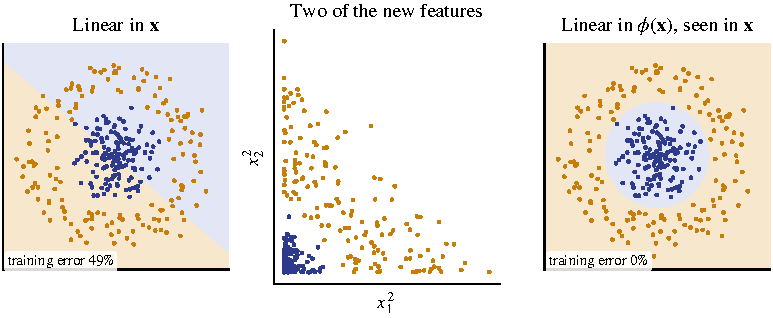
\includegraphics[width=\linewidth]{figures/feature_map.pdf}
\caption{Left: logistic regression on the raw inputs, 300 points. Centre: two of the five quadratic features,
$x_1^2$ and $x_2^2$, in which the classes are separated by a straight line. Right: logistic regression on the
five features $(x_1, x_2, x_1^2, x_1x_2, x_2^2)$, with the boundary drawn in the original coordinates.}
\label{fig:fmap}
\end{figure}

\section{Explicit feature maps}\label{sec:explicit}

\paragraph{Polynomial maps} The boundary in Figure~\ref{fig:fmap} is close to a circle, $x_1^2 + x_2^2 = r^2$. That
equation is not linear in $(x_1, x_2)$, but it is linear in the squares: with $u_1 = x_1^2$ and $u_2 = x_2^2$ it is the
straight line $u_1 + u_2 = r^2$ of the centre panel. The same holds for every conic. Write a general second-degree
polynomial with coefficients $c_{jk}$ indexed by the powers of $x_1$ and $x_2$:
\[
  c_{10}x_1 + c_{01}x_2 + c_{20}x_1^2 + c_{11}x_1x_2 + c_{02}x_2^2 + c_{00} = \w\T\phi(\x) + b, \qquad
  \phi(\x) = (x_1,\ x_2,\ x_1^2,\ x_1x_2,\ x_2^2) ,
\]
with $\w = (c_{10}, c_{01}, c_{20}, c_{11}, c_{02})$ and $b = c_{00}$. A polynomial in $\x$ is a \emph{linear} function
of its monomials, so fitting it is linear regression or linear classification on $\phi(\x)$, and the boundary
$\w\T\phi(\x) + b = 0$ can be any conic: ellipse, parabola, hyperbola or a pair of lines. Degree-$p$ maps give
boundaries that are algebraic curves of degree at most~$p$.

\paragraph{Counting the features} How large is $D$? A monomial $x_1^{k_1}\cdots x_d^{k_d}$ has degree $k_1 + \dots +
k_d$. Add a dummy variable $x_0 = 1$: monomials of degree \emph{at most} $p$ in $x_1, \dots, x_d$ correspond one to one
to monomials of degree \emph{exactly} $p$ in $x_0, x_1, \dots, x_d$ (the power of $x_0$ makes up the difference). A
monomial of degree exactly $p$ in $d+1$ variables is a way of placing $p$ identical balls into $d+1$ boxes, and there
are $\binom{d+p}{p}$ of those (``stars and bars'': arrange $p$ stars and $d$ separating bars in a row of $d + p$
symbols; the stars before the first bar are the power of $x_0$, those between the first and second bar the power of
$x_1$, and so on, and a row is fixed by choosing which $p$ of the $d + p$ positions hold stars). Hence
\begin{equation}\label{eq:count}
  D = \binom{d+p}{p} \quad \text{monomials of degree at most } p, \text{ including the constant.}
\end{equation}
In this note $D$ counts the constant monomial; when a separate bias $b$ is kept, as in Figure~\ref{fig:fmap}, the map
itself has the $D - 1$ non-constant components. Table~\ref{tab:count} shows how fast $D$ grows. For fixed $p$ it grows
like $d^p/p!$; a $28 \times 28$ image ($d = 784$) with cubic features needs eighty million of them. One sometimes reads
the cruder estimate $d^p$: that is the number of \emph{ordered} products $x_{j_1}x_{j_2}\cdots x_{j_p}$, which counts
$x_1x_2$ and $x_2x_1$ separately. For $d = 100$ and $p = 5$ it gives $10^{10}$, while merging equal monomials divides
it by roughly $p! = 120$ and leaves the $\approx 10^8$ of Table~\ref{tab:count}. The factors $\sqrt2$ in Worked
example~3 are what remains of this merging.

\begin{table}[h]
\centering\small
\caption{Number of polynomial features $D = \binom{d+p}{p}$ (constant included).}
\label{tab:count}
\begin{tabular}{@{}rrrr@{}}
\toprule
& $p = 2$ & $p = 3$ & $p = 5$ \\
\midrule
$d = 2$ & 6 & 10 & 21 \\
$d = 10$ & 66 & 286 & 3\,003 \\
$d = 100$ & 5\,151 & 176\,851 & 96\,560\,646 \\
$d = 784$ & 308\,505 & 80\,931\,145 & $\approx 2.5 \times 10^{12}$ \\
\bottomrule
\end{tabular}
\end{table}

\paragraph{What explicit maps cost} Three things grow with $D$. \emph{Memory}: storing $\phi(\x_i)$ for $n$ examples
takes $nD$ numbers; for $n = 10^4$, $d = 100$, $p = 3$ that is $1.8 \times 10^9$ numbers, about 7~GB in 32-bit floats.
\emph{Time}: every gradient step of logistic regression or every pass of the perceptron touches all $nD$ numbers.
\emph{Capacity}: the model has $D$ parameters (the constant monomial plays the role of the bias; the quadratic map in
the plane has $D = 6$: five features plus the bias) and can overfit, so regularisation (Note~4, Section~7) and more data
are needed --- the curse of dimensionality (Note~3, Section~3) in a new form.

Polynomials are not the only explicit choice. Physically motivated variables (an invariant mass, an energy, a radius
$\norm{\x}$), Fourier features $\sin(\vect{\omega}\T\x)$ and $\cos(\vect{\omega}\T\x)$, and random non-linear features
(the random ReLU features of Note~4, Section~8) are all feature maps. Algorithm~\ref{alg:explicit} is the same for all
of them.

\begin{algorithm}[htbp]
\caption{Explicit feature map followed by a linear classifier}\label{alg:explicit}
\begin{algorithmic}[1]
\Require training set $\{(\x_i, t_i)\}_{i=1}^n$, $\x_i \in \R^d$, $t_i \in \{-1,+1\}$; feature map $\phi : \R^d \to \R^D$;
  a linear training algorithm \textsc{LinearFit} (any of Note~9)
\Function{ExplicitFit}{$\{(\x_i, t_i)\}$}
  \For{$i = 1, \dots, n$}
    \State row $i$ of $\Phi$ $\gets \phi(\x_i)\T$ \Comment{$O(D)$ for a polynomial map}
  \EndFor
  \State $(\w, b) \gets \textsc{LinearFit}(\Phi, \vect{t})$ \Comment{e.g.\ perceptron, logistic regression, linear SVM}
  \State \Return $(\w, b)$
\EndFunction
\Function{ExplicitPredict}{$\x$; $\w, b$}
  \State \Return $\operatorname{sign}\big(\w\T\phi(\x) + b\big)$
\EndFunction
\end{algorithmic}
\end{algorithm}

\begin{runtime}{explicit feature map + linear classifier}
\emph{Training}: computing the features costs $O(nD)$ (each monomial is one product of a lower-degree monomial and one
coordinate); $T$ passes of gradient descent or of the perceptron cost $O(TnD)$; a closed-form least-squares classifier costs
$O(nD^2 + D^3)$ (forming and solving the $D \times D$ normal equations, Note~8). \emph{Prediction}: $O(D)$ per query,
for $\phi(\x)$ and one dot product. \emph{Memory}: $O(nD)$ for the mapped data, or $O(D)$ if features are recomputed
on the fly in each pass. With $D = \binom{d+p}{p}$ this is fine up to $D \sim 10^5$ and hopeless beyond $10^7$.
\end{runtime}

\begin{worked}{2. A perceptron on explicit quadratic features}
Three points on a line, $x = -1, 0, 2$, with labels $t = +1, -1, +1$: the negative point sits between the two positive
ones, so no single threshold on $x$ separates them. Map each point to $\phi(x) = (x, x^2)$, giving $(-1, 1)$, $(0, 0)$
and $(2, 4)$, and run the perceptron of Note~9, Section~3, with a bias: start from $\w = (0, 0)$, $b = 0$, and on a
mistake ($t\,g \le 0$ with $g = \w\T\phi(x) + b$) set $\w \gets \w + t\,\phi(x)$, $b \gets b + t$.
\begin{center}\small
\begin{tabular}{@{}cccccll@{}}
\toprule
pass & $x$ & $t$ & $\phi(x)$ & $g$ (before update) & result & $(\w;\ b)$ after \\
\midrule
1 & $-1$ & $+1$ & $(-1, 1)$ & $0$ & mistake & $(-1, 1;\ 1)$ \\
1 & $0$ & $-1$ & $(0, 0)$ & $1$ & mistake & $(-1, 1;\ 0)$ \\
1 & $2$ & $+1$ & $(2, 4)$ & $-2 + 4 + 0 = 2$ & correct & \\
2 & $-1$ & $+1$ & $(-1, 1)$ & $1 + 1 + 0 = 2$ & correct & \\
2 & $0$ & $-1$ & $(0, 0)$ & $0$ & mistake & $(-1, 1;\ -1)$ \\
2 & $2$ & $+1$ & $(2, 4)$ & $1$ & correct & \\
3 & all & & & $1, -1, 1$ & all correct & converged \\
\bottomrule
\end{tabular}
\end{center}
After three mistakes the perceptron stops with $\w = (-1, 1)$ and $b = -1$, a straight line in the $(x, x^2)$ plane.
Read in the input space it is the quadratic
\[
  g(x) = x^2 - x - 1 ,
\]
whose roots $x = (1 \pm \sqrt5)/2 \approx -0.618$ and $1.618$ are the decision boundary: points between them are
classified $-1$, points outside $+1$. The algorithm never knew it was fitting a parabola; it saw only two-dimensional
vectors. Question~B3 runs the kernel version of the perceptron on a similar problem.
\end{worked}

\paragraph{Three routes to non-linearity} The feature map can be fixed in advance and computed, fixed in advance but
never computed, or fitted to the data. The routes differ in what the designer chooses, what training adjusts, and
what the cost grows with:
\begin{center}\small
\begin{tabular}{@{}L{0.2\linewidth}L{0.25\linewidth}L{0.22\linewidth}L{0.24\linewidth}@{}}
\toprule
route & chosen by hand & fitted to data & cost grows with \\
\midrule
explicit map (this section) & $\phi$ itself & $\w \in \R^D$ & $D$, the number of features \\
kernel (Sections~\ref{sec:trick}--\ref{sec:family}) & $k(\x, \z) = \phi(\x)\T\phi(\z)$ & $n$ coefficients $\alpha_i$ & $n$, through an
$n \times n$ matrix \\
learned features (week~5) & the form of $\phi$, e.g.\ $a(V\x + \vect{c})$ & $V$, $\vect{c}$ and $\w$ together & the number of
parameters; non-convex training \\
\bottomrule
\end{tabular}
\end{center}
In the third row $a$ is an element-wise non-linearity and $V$ a matrix trained by gradient descent (Note~7) with $\w$: a
multilayer perceptron is a linear model on features that are themselves learned.

\section{The kernel trick}\label{sec:trick}

\subsection{Algorithms that need only dot products}

Note~9, Section~3 (``The dual form'') showed that the perceptron's weight vector is a sum of the training inputs weighted
by mistake counts. Here we drop the bias (it returns below as $k + 1$) and run the same algorithm on the mapped inputs
$\phi(\x_i)$. It starts from $\w = \vect{0}$ and, on each mistake on example $i$, adds $t_i\phi(\x_i)$ to $\w$. After
training, therefore,
\begin{equation}\label{eq:repr}
  \w = \sum_{i=1}^n \alpha_i t_i\, \phi(\x_i), \qquad \alpha_i = \text{number of mistakes made on example } i .
\end{equation}
The weight vector is a combination of the training inputs, and the $n$ integers $\alpha_i$ describe it completely,
whatever the dimension $D$. Its score on any input is
\begin{equation}\label{eq:kscore}
  g(\x) = \w\T\phi(\x) = \sum_{i=1}^n \alpha_i t_i\, \phi(\x_i)\T\phi(\x) = \sum_{i=1}^n \alpha_i t_i\, k(\x_i, \x),
\end{equation}
where the \emph{kernel}
\begin{equation}\label{eq:kernel}
  k(\x, \z) = \phi(\x)\T\phi(\z)
\end{equation}
is the dot product in feature space. Training needs the scores $g(\x_j)$ on training points, hence only the numbers
$k(\x_i, \x_j)$, collected in the $n \times n$ \emph{Gram matrix} $K_{ij} = k(\x_i, \x_j)$; prediction needs only
$k(\x_i, \x)$. If $k$ can be evaluated without computing $\phi$, the algorithm runs in feature space without ever
visiting it. That is the kernel trick~\cite{aizerman1964,boser1992}.

\paragraph{Why the weight vector lies in the span of the data} Equation~\eqref{eq:repr} is not a peculiarity of the
perceptron. Consider any objective of the form
\[
  J(\w) = L\big(\w\T\phi(\x_1), \dots, \w\T\phi(\x_n)\big) + \lambda\norm{\w}^2 , \qquad \lambda > 0,
\]
where $L$ is any loss that depends on $\w$ only through the scores on the training points --- squared error, logistic
loss, hinge loss. Split $\w = \w_\parallel + \w_\perp$, with $\w_\parallel$ in the span of
$\phi(\x_1), \dots, \phi(\x_n)$ and $\w_\perp$ orthogonal to all of them. Then $\w\T\phi(\x_i) = \w_\parallel\T\phi(\x_i)$
for every $i$, so $L$ does not see $\w_\perp$, while $\norm{\w}^2 = \norm{\w_\parallel}^2 + \norm{\w_\perp}^2$ is smallest
for $\w_\perp = \vect{0}$. The minimiser therefore has the form $\w = \sum_i \beta_i \phi(\x_i)$. This is the
\emph{representer theorem}~\cite{kimeldorf1971,scholkopf2001}; it covers ridge regression, regularised logistic regression
and the SVM.

\paragraph{Kernelising in practice} Every method in this note is obtained the same way. Examples must meet only in
pairs, through $\x_i\T\x_j$ during training and $\x_i\T\x$ at prediction; the algorithm keeps track of the $n$
coefficients of $\w$ in the span of the data instead of $\w$ itself; and each pairwise dot product is evaluated as
$k(\x_i, \x_j)$. Nothing is approximated: the kernelised algorithm produces exactly the iterates that the original one
would produce on the points $\phi(\x_i)$. The mapping must happen \emph{before} the algorithm runs, because $\phi$ is
non-linear and does not commute with taking combinations: $\sum_i \beta_i\phi(\x_i)$ is in general not the image
$\phi(\vect{v})$ of any input point $\vect{v}$, let alone of $\sum_i \beta_i\x_i$ (Worked example~4 shows a case).

\subsection{Computing a dot product without the features}

\begin{worked}{3. Two polynomial kernels, checked by hand}
\emph{The homogeneous quadratic kernel.} For $\x, \z \in \R^2$ expand
\[
  (\x\T\z)^2 = (x_1z_1 + x_2z_2)^2 = x_1^2z_1^2 + 2x_1x_2z_1z_2 + x_2^2z_2^2 = \phi(\x)\T\phi(\z), \qquad
  \phi(\x) = \big(x_1^2,\ \sqrt2\,x_1x_2,\ x_2^2\big).
\]
The factor $\sqrt2$ appears because the cross term occurs twice. Take $\x = (1, 2)$ and $\z = (3, 1)$. With the
kernel: $\x\T\z = 3 + 2 = 5$, so $k(\x, \z) = 25$. With the features,
\[
  \phi(\x) = (1,\ 2\sqrt2,\ 4), \quad \phi(\z) = (9,\ 3\sqrt2,\ 1), \quad
  \phi(\x)\T\phi(\z) = 9 + 2\sqrt2 \cdot 3\sqrt2 + 4 = 9 + 12 + 4 = 25 .
\]
\emph{The inhomogeneous quadratic kernel.} Expanding $(1 + \x\T\z)^2 = 1 + 2\x\T\z + (\x\T\z)^2$ gives a six-dimensional
map,
\[
  \phi(\x) = \big(1,\ \sqrt2\,x_1,\ \sqrt2\,x_2,\ x_1^2,\ \sqrt2\,x_1x_2,\ x_2^2\big),
\]
which contains all $\binom{2+2}{2} = 6$ monomials of degree at most two, with weights. For the same points the kernel
gives $k(\x, \z) = (1 + 5)^2 = 36$, while
\[
  \phi(\x) = (1, \sqrt2, 2\sqrt2, 1, 2\sqrt2, 4), \qquad \phi(\z) = (1, 3\sqrt2, \sqrt2, 9, 3\sqrt2, 1),
\]
and the six products sum to $\phi(\x)\T\phi(\z) = 1 + 6 + 4 + 9 + 12 + 4 = 36$.

\emph{The costs.} The kernel needs one $d$-dimensional dot product, one addition and one squaring: about $d + 2$
operations. The features need $D$ operations for each $\phi$ and $D$ more for the dot product. For $(1 + \x\T\z)^p$
with $d = 100$ and $p = 3$, that is about $10^2$ operations against $3 \times 176\,851 \approx 5 \times 10^5$, a factor of
several thousand, and the gap widens with $p$.
\end{worked}

The same expansion works in general: by the multinomial theorem, $(c + \x\T\z)^p$ with $c > 0$ is the dot product of
two vectors containing all $\binom{d+p}{p}$ monomials of degree at most $p$, each multiplied by the square root of a
positive coefficient; $(\x\T\z)^p$ contains only the monomials of degree exactly $p$. A degree-$p$ polynomial classifier
can thus be trained at cost $O(d)$ per kernel evaluation instead of $O(d^p)$.

\subsection{The kernel perceptron}

Combining \eqref{eq:repr} and \eqref{eq:kscore} turns the perceptron into an algorithm on the mistake counts
$\alpha_i$~\cite{aizerman1964,freund1999}. The mistake test for example $j$, $t_j\,\w\T\phi(\x_j) \le 0$, becomes
$t_j\sum_i \alpha_i t_i K_{ij} \le 0$, and the update $\w \gets \w + t_j\phi(\x_j)$ becomes $\alpha_j \gets \alpha_j + 1$.

\paragraph{A bias for free} The linear perceptron also updates a bias, $b \gets b + t_j$. The bias starts at $0$ and
gains $t_i$ on every mistake on example $i$, so in the kernel version it equals $b = \sum_i \alpha_i t_i$, and $g(\x) + b = \sum_i \alpha_i t_i\,[k(\x_i, \x) + 1]$: keeping a bias is the
same as replacing $k$ by $k + 1$, which appends a constant feature to $\phi$. The kernel $(1 + \x\T\z)^p$ already
contains one.

\begin{algorithm}[htbp]
\caption{Kernel perceptron}\label{alg:kperc}
\begin{algorithmic}[1]
\Require training set $\{(\x_i, t_i)\}_{i=1}^n$, $t_i \in \{-1,+1\}$; kernel $k$; maximum number of passes $T$
\Ensure mistake counts $\alpha_1, \dots, \alpha_n$
\Function{KernelPerceptronFit}{$\{(\x_i, t_i)\}$, $k$, $T$}
  \State $K \gets \textsc{Gram}(\x_1, \dots, \x_n; k)$ \Comment{Algorithm~\ref{alg:gram}, $O(n^2 d)$}
  \State $\alpha_i \gets 0$ for all $i$
  \For{pass $= 1, \dots, T$}
    \State mistakes $\gets 0$
    \For{$j = 1, \dots, n$} \Comment{or in random order}
      \State $g_j \gets \sum_{i : \alpha_i > 0} \alpha_i t_i K_{ij}$ \Comment{score of $\x_j$, $O(n)$}
      \If{$t_j g_j \le 0$}
        \State $\alpha_j \gets \alpha_j + 1$; \ mistakes $\gets$ mistakes $+ 1$
      \EndIf
    \EndFor
    \If{mistakes $= 0$} \textbf{break} \EndIf
  \EndFor
  \State \Return $\valpha$
\EndFunction
\Function{KernelPerceptronPredict}{$\x$; $\{(\x_i, t_i, \alpha_i)\}$, $k$}
  \State \Return $\operatorname{sign}\big(\sum_{i : \alpha_i > 0} \alpha_i t_i\, k(\x_i, \x)\big)$
\EndFunction
\end{algorithmic}
\end{algorithm}

\begin{runtime}{kernel perceptron}
\emph{Training}: the Gram matrix costs $O(n^2 d)$ once ($n^2$ kernel values at $O(d)$ each); each score $g_j$ is a sum
over at most $n$ terms, so one pass costs $O(n^2)$ and $T$ passes $O(n^2(d + T))$. \emph{Memory}: $O(n^2)$ for $K$;
without storing $K$, recompute kernel values on demand, $O(nd)$ memory and $O(Tn\,M d)$ time, where $M$ is the number of
examples with $\alpha_i > 0$. \emph{Prediction}: $O(M d)$ per query, one kernel evaluation per stored example. If the
mapped data are separable with margin $\gamma$ by a hyperplane through the origin of feature space (or, when a bias is
kept, with $k$ replaced by $k + 1$), Novikoff's bound (Note~9, Section~3) applies with $R^2 = \max_i k(\x_i, \x_i)$: the
total number of mistakes --- and hence $M$ --- is at most $(R/\gamma)^2$, independent of $D$.
\end{runtime}

\begin{worked}{4. The kernel perceptron solves XOR}
Use the centred XOR points of Section~\ref{sec:why} and the kernel $k(\x, \z) = (1 + \x\T\z)^2$. From now on we write
$\x = (x_1, x_2)$ for the centred coordinates $(s_1, s_2)$ of Worked example~1; bold $\x_1, \dots, \x_4$ label the four
points.
\[
\begin{array}{c|cccc}
 & \x_1 & \x_2 & \x_3 & \x_4 \\ \hline
 \x & (1, 1) & (-1, -1) & (1, -1) & (-1, 1) \\
 t & +1 & +1 & -1 & -1
\end{array}
\]
\emph{Gram matrix.} Each point has $\x_i\T\x_i = 2$, so $K_{ii} = (1 + 2)^2 = 9$. Neighbouring points have $\x_i\T\x_j = 0$
and opposite points $\x_i\T\x_j = -2$; both give $K_{ij} = 1$. Hence $K = 8I + \vect{1}\vect{1}\T$: nines on the diagonal,
ones elsewhere, and the score of $\x_j$ is
\[
  g_j = \sum_i \alpha_i t_i K_{ij} = 8\,\alpha_j t_j + S, \qquad S = \sum_i \alpha_i t_i .
\]
\noindent\begin{minipage}{\linewidth}
\emph{Trace.} Visit the points in the order $1, 2, 3, 4$ and update when $t_j g_j \le 0$. The column $g_j$ shows the
two terms $8\alpha_jt_j$ and $S$, evaluated before the update:
\begin{center}\small
\begin{tabular}{@{}cccrccl@{}}
\toprule
pass & $j$ & $t_j$ & $g_j = 8\alpha_jt_j + S$ & $t_jg_j \le 0$\,? & $\valpha$ after & \\
\midrule
1 & 1 & $+1$ & $0$ & mistake & $(1,0,0,0)$ & start: all scores zero \\
1 & 2 & $+1$ & $0 + 1 = 1$ & no & $(1,0,0,0)$ & \\
1 & 3 & $-1$ & $0 + 1 = 1$ & mistake & $(1,0,1,0)$ & $S$ becomes $0$ \\
1 & 4 & $-1$ & $0 + 0 = 0$ & mistake & $(1,0,1,1)$ & $S$ becomes $-1$ \\
2 & 1 & $+1$ & $8 - 1 = 7$ & no & & \\
2 & 2 & $+1$ & $0 - 1 = -1$ & mistake & $(1,1,1,1)$ & $S$ becomes $0$ \\
2 & 3 & $-1$ & $-8 + 0 = -8$ & no & & \\
2 & 4 & $-1$ & $-8 + 0 = -8$ & no & & \\
3 & 1--4 & & $8, 8, -8, -8$ & no & $(1,1,1,1)$ & converged \\
\bottomrule
\end{tabular}
\end{center}
\end{minipage}
\smallskip

\noindent After four mistakes every point is classified correctly, with $\valpha = (1, 1, 1, 1)$.

\emph{The decision function.} Put $u = x_1 + x_2$ and $v = x_1 - x_2$. Then $\x_1\T\x = u$, $\x_2\T\x = -u$,
$\x_3\T\x = v$ and $\x_4\T\x = -v$, so with all $\alpha_i = 1$ the score $g(\x) = \sum_i \alpha_it_i(1 + \x_i\T\x)^2$ is
\[
  g(\x) = (1 + u)^2 + (1 - u)^2 - (1 + v)^2 - (1 - v)^2 = 2u^2 - 2v^2 = 8\,x_1x_2 .
\]
The kernel perceptron has found the sign of the product, the function of Section~\ref{sec:why}, without ever forming a
product feature. At a new point, $g(0.5, 0.5) = 2$ and $g(2, -1) = -16$.

\emph{What happened in feature space.} With the six features of Worked example~3, $\w = \sum_i \alpha_i t_i\phi(\x_i)$:
the constant, linear and squared components cancel in pairs and only the cross feature survives,
$\w = (0, 0, 0, 0, 4\sqrt2, 0)$, so $\w\T\phi(\x) = 4\sqrt2 \cdot \sqrt2\,x_1x_2 = 8x_1x_2$. Combining the inputs first
and mapping afterwards gives something else entirely: $\sum_i \alpha_i t_i \x_i = (0, 0)$ and $\phi(0, 0) = (1, 0, 0, 0,
0, 0)$, a constant classifier. In fact no input $\vect{v}$ has $\phi(\vect{v}) = \w$, since the first component of
$\phi(\vect{v})$ is always $1$.

\emph{The mistake bound.} Every point has $\norm{\phi(\x_i)}^2 = K_{ii} = 9$, so $R = 3$. The unit vector along the cross
feature, a hyperplane through the origin of feature space, separates the data with margin $t_i\sqrt2\,x_{i1}x_{i2} =
\sqrt2$. Novikoff's bound allows at most
$(R/\gamma)^2 = 9/2$ mistakes; we made four.
\end{worked}

\paragraph{Computing the Gram matrix} Every kernel method starts by filling $K$. For the Gaussian kernel of the next
section, the identity $\norm{\x_i - \x_j}^2 = \norm{\x_i}^2 + \norm{\x_j}^2 - 2\x_i\T\x_j$ (Note~1, Section~6) turns all
squared distances into one matrix product $XX\T$.

\begin{algorithm}[htbp]
\caption{Gram matrix (vectorised)}\label{alg:gram}
\begin{algorithmic}[1]
\Require data matrix $X \in \R^{n \times d}$ (rows $\x_i\T$), kernel $k$
\Function{Gram}{$X$; $k$}
  \State $P \gets XX\T$ \Comment{all dot products, $O(n^2 d)$}
  \If{$k$ is polynomial, $(c + \x\T\z)^p$}
    \State $K \gets (c + P)^{\circ p}$ \Comment{element-wise power}
  \ElsIf{$k$ is Gaussian with width $\sigma$}
    \State $\vect{q} \gets \operatorname{diag}(P)$ \Comment{squared norms $\norm{\x_i}^2$}
    \State $K_{ij} \gets \exp\!\big(-(q_i + q_j - 2P_{ij}) / (2\sigma^2)\big)$ for all $i, j$
  \Else
    \State $K_{ij} \gets k(\x_i, \x_j)$ for all $i \le j$; \ $K_{ji} \gets K_{ij}$ \Comment{any other kernel}
  \EndIf
  \State \Return $K$ \Comment{symmetric: only $n(n+1)/2$ distinct entries}
\EndFunction
\end{algorithmic}
\end{algorithm}

\begin{runtime}{Gram matrix}
\emph{Time}: $O(n^2 d)$, dominated by $XX\T$, a single matrix product that BLAS libraries and GPUs execute at close to
peak speed; the element-wise step adds $O(n^2)$. \emph{Memory}: $O(n^2)$: $10^8$ numbers or 0.8~GB in 64-bit floats for
$n = 10^4$; 80~GB for $n = 10^5$; 8~TB for $n = 10^6$. Memory, not time, usually limits exact kernel methods. A test
block $K(X_{\mathrm{test}}, X)$ costs $O(n_{\mathrm{test}}\, n\, d)$.
\end{runtime}

\section{Common kernels}\label{sec:common}

\paragraph{Linear} $k(\x, \z) = \x\T\z$, with $\phi(\x) = \x$. It reproduces the original linear algorithm; kernelising
with it is useful only when $d > n$, where the $n \times n$ Gram matrix is smaller than the $d \times d$ matrices of the
primal form.

\paragraph{Polynomial} $k(\x, \z) = (c + \x\T\z)^p$ with $c \ge 0$ and integer $p \ge 1$: all monomials of degree at most
$p$ ($c > 0$) or exactly $p$ ($c = 0$). The constant $c$ sets the weight of low-degree terms relative to high-degree
ones. For large inputs $k$ grows like $(\norm{\x}\,\norm{\z})^p$ (so $k(\x, \x) \sim \norm{\x}^{2p}$), and a large $p$
quickly produces huge or tiny numbers, so inputs must be scaled to modest norms. The degree $p$ and the constant $c$
are hyperparameters, chosen together with the regularisation constant by validation (Note~4, Section~7).

\paragraph{Gaussian or radial basis function (RBF)}
\begin{equation}\label{eq:rbf}
  k_\sigma(\x, \z) = \exp\!\left(-\frac{\norm{\x - \z}^2}{2\sigma^2}\right).
\end{equation}
It equals $1$ when $\x = \z$ and falls to $0$ as the points move apart, on the length scale $\sigma$: a similarity
measure. It depends only on $\x - \z$ (it is \emph{stationary}, or translation invariant), and is by far the most common
default. Its feature space is infinite-dimensional.

\begin{worked}{5. The Gaussian kernel has infinitely many features}
In one dimension, factor the exponent: $-(x - z)^2/(2\sigma^2) = -x^2/(2\sigma^2) - z^2/(2\sigma^2) + xz/\sigma^2$, so
\[
  k_\sigma(x, z) = e^{-x^2/2\sigma^2}\, e^{-z^2/2\sigma^2}\, e^{xz/\sigma^2}
  = e^{-x^2/2\sigma^2}\, e^{-z^2/2\sigma^2} \sum_{m=0}^\infty \frac{1}{m!}\left(\frac{xz}{\sigma^2}\right)^{\!m} ,
\]
using the Taylor series $e^u = \sum_m u^m/m!$. Each term splits into a function of $x$ times the same function of $z$:
\[
  k_\sigma(x, z) = \sum_{m=0}^\infty \phi_m(x)\,\phi_m(z), \qquad
  \phi_m(x) = e^{-x^2/2\sigma^2}\, \frac{x^m}{\sigma^m\sqrt{m!}} .
\]
The feature map $\phi(x) = (\phi_0(x), \phi_1(x), \phi_2(x), \dots)$ has infinitely many components: every power of
$x$, damped by a Gaussian envelope and by $1/\sqrt{m!}$.

\emph{Numerically.} Take $x = 1$, $z = 0.5$, $\sigma = 1$. Exactly, $k = e^{-0.125} = 0.8825$. The prefactor is
$e^{-0.5}e^{-0.125} = 0.5353$, and keeping the terms $m = 0, 1, \dots, m_{\max}$ of the series gives
\[
\begin{array}{c|cccccc}
m_{\max} & 0 & 1 & 2 & 3 & 4 & 5 \\ \hline
\text{partial sum} & 0.5353 & 0.8029 & 0.8698 & 0.8810 & 0.8823 & 0.8825
\end{array}
\]
The series converges quickly here, but no finite truncation is exact for all $x, z$, and the kernel evaluates the
infinite sum in one exponential. In $d$ dimensions $k_\sigma$ is the product of $d$ such one-dimensional kernels, because
$\norm{\x - \z}^2 = \sum_j (x_j - z_j)^2$ and the exponential of a sum is the product of the exponentials. A product of
kernels has as features all pairwise products of their features (Section~\ref{sec:mercer}, rule~3), so the features of
$k_\sigma$ are all monomials of all degrees, each with its Gaussian envelope.
\end{worked}

\paragraph{The width $\sigma$} The width is the most important hyperparameter of the Gaussian kernel. As $\sigma \to 0$,
$K \to I$: each training point is similar only to itself, the model can memorise any labelling, and the boundary breaks
into small islands around individual points. As $\sigma \to \infty$, all kernel values approach $1$ and differ only
through the small term $-\norm{\x - \z}^2/(2\sigma^2)$. In the Taylor series of Worked example~5 the terms of degree $m$
carry a factor $\sigma^{-2m}$, so only the first few powers matter: the model behaves like a low-degree polynomial
classifier and cannot follow a strongly curved boundary. Figure~\ref{fig:kwidths} shows both extremes and a good
compromise on the two-moons data (the classifier used there, the kernel SVM, comes in Section~\ref{sec:ksvm}). Choose $\sigma$, together with the regularisation constant, by cross-validation
(Note~4, Sections~4 and~7); a common starting point is the median distance between training points. Because the kernel
depends on Euclidean distances, standardise the features first (Note~5, Section~5).

\begin{figure}[htbp]
\centering
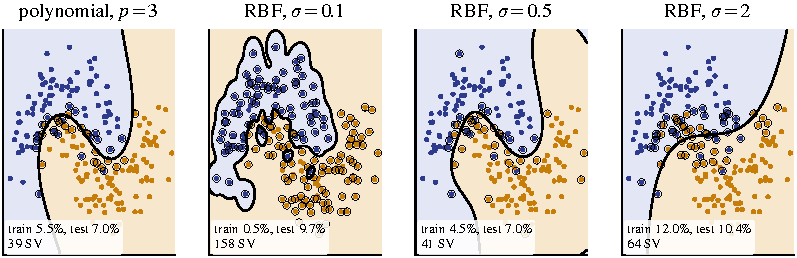
\includegraphics[width=\linewidth]{figures/n10_kernel_widths.pdf}
\caption{Kernel SVMs ($C = 10$) on 200 points of the two-moons data, trained by Algorithm~\ref{alg:ksvm} (bias absorbed
by adding 1 to the kernel, as in ``A bias for free''); test errors on 2000 new points. The kernel SVM, its constant $C$
and its support vectors (circled) are explained in Section~\ref{sec:ksvm}; here only the shape of the boundary
matters. A cubic polynomial kernel, $(1 + \x\T\z)^3$, and a Gaussian kernel of width
$\sigma = 0.5$ both reach 7.0\% test error. The narrow Gaussian ($\sigma = 0.1$) fits the training set almost perfectly
(0.5\%) but draws islands, uses 158 of the 200 points as support vectors and reaches 9.7\% test error; the wide one
($\sigma = 2$) is too smooth (12.0\% training, 10.4\% test error).}
\label{fig:kwidths}
\end{figure}

Many other kernels exist: the Laplacian kernel $\exp(-\norm{\x - \z}/\sigma)$, kernels that compare strings by their
common substrings (used for DNA and protein sequences), kernels on trees (for instance the parse trees of sentences in
language processing), on graphs and on sets. What they share is the property of
the next section.

\section{What makes a valid kernel}\label{sec:mercer}

A function $k(\x, \z)$ is a \emph{kernel} if there exists a feature map $\phi$, into $\R^D$ or into an
infinite-dimensional space with a dot product, such that $k(\x, \z) = \phi(\x)\T\phi(\z)$ for all $\x, \z$. Not every
similarity function qualifies.

\paragraph{A necessary condition} Take any points $\x_1, \dots, \x_n$ and any real coefficients $c_1, \dots, c_n$.
If $k$ is a kernel,
\[
  \vect{c}\T K\vect{c} = \sum_{i,j} c_ic_j\, \phi(\x_i)\T\phi(\x_j)
  = \Big(\sum_i c_i\phi(\x_i)\Big)\T\Big(\sum_j c_j\phi(\x_j)\Big) = \Big\lVert \sum_i c_i\phi(\x_i)\Big\rVert^2 \ge 0 .
\]
So every Gram matrix of a kernel is symmetric and \emph{positive semi-definite} (PSD): $\vect{c}\T K\vect{c} \ge 0$ for all
$\vect{c}$, equivalently all its eigenvalues are non-negative. A squared length cannot be negative.

\paragraph{The converse (Moore--Aronszajn, Mercer)} The condition is also sufficient: a symmetric function $k$ for which
every Gram matrix, on any finite set of points, is PSD is a kernel for some feature map $\phi$. In this form the result is
the reproducing-kernel Hilbert-space construction usually credited to Moore and Aronszajn; Mercer's 1909 theorem is the
continuous version, for continuous $k$ on a compact domain, with $\phi$ built from the eigenfunctions of
$k$~\cite{mercer1909,scholkopf2002}. (These constructions are beyond this course; all we use is the statement: a
symmetric $k$ is a valid kernel exactly when all its Gram matrices are PSD.) Kernels with this property are therefore
often called Mercer kernels. This is why one
can use the Gaussian kernel without ever writing its features: it is enough to know that its Gram matrices are PSD.

\begin{worked}{6. Checking a Gram matrix}
\emph{A valid kernel.} Take the one-dimensional points $x = 0, 1, 2$ and $k(x, z) = (1 + xz)^2$:
\[
  K = \begin{pmatrix} 1 & 1 & 1 \\ 1 & 4 & 9 \\ 1 & 9 & 25 \end{pmatrix}.
\]
It is symmetric. Its \emph{leading principal minors} are the determinants of its top-left $1 \times 1$, $2 \times 2$
and $3 \times 3$ sub-matrices; for a symmetric matrix, if all of them are positive the matrix is positive definite
(Sylvester's criterion), and hence PSD. Here $1 > 0$, \ $1 \cdot 4 - 1 \cdot 1 = 3 > 0$ and
$\det K = 1(100 - 81) - 1(25 - 9) + 1(9 - 4) = 19 - 16 + 5 = 8 > 0$. Numerically the eigenvalues are $0.200$, $1.411$
and $28.390$, all positive, as they must be. (The test only works in this direction: a minor equal to zero does not
settle the question, and then one checks the eigenvalues instead.)

\emph{Not a kernel.} The squared distance $k(\x, \z) = \norm{\x - \z}^2$ is symmetric and non-negative, a reasonable
``dissimilarity''. On the two points $0$ and $1$ its Gram matrix is $\begin{pmatrix} 0 & 1 \\ 1 & 0 \end{pmatrix}$, and
with $\vect{c} = (1, -1)$, $\vect{c}\T K\vect{c} = 0 - 1 - 1 + 0 = -2 < 0$: it would be a vector of negative squared
length. Its eigenvalues are $\pm 1$. (Its negative, $-\norm{\x - \z}^2$, fails too, with $\vect{c} = (1, 1)$.)
\end{worked}

A non-PSD ``kernel'' is not only a theoretical flaw: the dual SVM problem then stops being concave, so solvers can get
stuck in local maxima (and for the hard margin the objective can be unbounded), and $K + \lambda I$ in kernel ridge
regression can become singular. The sigmoid function $\tanh(a\,\x\T\z + c)$, offered as a kernel in early SVM software,
is a well-known example: it is not positive semi-definite in general, although its Gram matrices happen to be PSD for
some parameter values on some data sets~\cite{scholkopf2002}.

\paragraph{Building kernels from kernels} Rather than check PSD-ness each time, build new kernels from known ones. If
$k_1$ and $k_2$ are kernels with feature maps $\phi_1$ and $\phi_2$, so are
\begin{enumerate}
\item $k_1 + k_2$: concatenate the features, $\phi = (\phi_1, \phi_2)$;
\item $c\,k_1$ for $c > 0$: scale the features, $\phi = \sqrt c\,\phi_1$;
\item $k_1 k_2$: take all pairwise products of features, $\phi_{ab}(\x) = \phi_{1,a}(\x)\,\phi_{2,b}(\x)$; then
  $\sum_{a,b}\phi_{ab}(\x)\phi_{ab}(\z) = \big(\sum_a \phi_{1,a}(\x)\phi_{1,a}(\z)\big)\big(\sum_b \phi_{2,b}(\x)\phi_{2,b}(\z)\big)
  = k_1k_2$;
\item $f(\x)\,k_1(\x, \z)\,f(\z)$ for any real function $f$: $\phi = f\phi_1$;
\item any polynomial in $k_1$ with non-negative coefficients (a constant $c \ge 0$ is itself a kernel, with the single
  feature $\sqrt c$), and $\exp(k_1)$, the limit of its Taylor polynomials: by rules 1--3, and because a pointwise limit of
  kernels is a kernel (a limit of PSD matrices is PSD);
\item $k_1(\psi(\x), \psi(\z))$ for any map $\psi$, for instance a preprocessing step.
\end{enumerate}
For example, $(1 + \x\T\z)^2 = 1 + 2\,\x\T\z + (\x\T\z)^2$ is valid by rules~1--3. The Gaussian kernel is valid because
$k_\sigma(\x, \z) = f(\x)\exp(\x\T\z/\sigma^2)f(\z)$ with $f(\x) = \exp(-\norm{\x}^2/2\sigma^2)$: $\x\T\z/\sigma^2$ is a
kernel by rule~2, its exponential by rule~5, and the product with $f$ by rule~4 --- the $d$-dimensional version of Worked
example~5.

\section{Kernel ridge regression}\label{sec:krr}

Ridge regression (Note~8, Section~4) kernelises in a few lines and gives the simplest complete kernel method. Map the
inputs, collect the features as the rows of $\Phi \in \R^{n \times D}$, and minimise
\begin{equation}\label{eq:ridgephi}
  J(\w) = \norm{\Phi\w - \y}^2 + \lambda\norm{\w}^2 .
\end{equation}
To keep the algebra short we drop the bias: centre the targets first (subtract their mean, add it back to predictions),
or add a constant to the kernel. The primal solution is $\w = (\Phi\T\Phi + \lambda I_D)^{-1}\Phi\T\y$, which needs a
$D \times D$ system --- impossible for the Gaussian kernel, where $D = \infty$.

\paragraph{Derivation through the representer form} Set the gradient of \eqref{eq:ridgephi} to zero:
\[
  2\Phi\T(\Phi\w - \y) + 2\lambda\w = \vect{0}
  \quad\Longrightarrow\quad
  \lambda\w = \Phi\T(\y - \Phi\w)
  \quad\Longrightarrow\quad
  \w = \Phi\T\valpha, \qquad \valpha = \frac{1}{\lambda}(\y - \Phi\w) .
\]
This defines $\valpha$ only implicitly, since $\w$ still appears on the right; the next step solves for it. Already,
however, $\w = \sum_i \alpha_i\phi(\x_i)$, as the representer theorem promised, with $\alpha_i$ proportional to the
residual of example $i$. (In regression there is no label factor: unlike the perceptron and the SVM, where
$\w = \sum_i \alpha_it_i\phi(\x_i)$, here $\w = \sum_i \alpha_i\phi(\x_i)$ and $\alpha_i$ carries its own sign.) Substitute $\w = \Phi\T\valpha$ into the definition of $\valpha$ and use $\Phi\Phi\T = K$ (the Gram
matrix, $(\Phi\Phi\T)_{ij} = \phi(\x_i)\T\phi(\x_j)$):
\[
  \lambda\valpha = \y - \Phi\Phi\T\valpha = \y - K\valpha
  \quad\Longrightarrow\quad
  (K + \lambda I_n)\,\valpha = \y
  \quad\Longrightarrow\quad
  \valpha = (K + \lambda I_n)^{-1}\y .
\]
The prediction at a new point is
\begin{equation}\label{eq:krrpred}
  f(\x) = \w\T\phi(\x) = \sum_{i=1}^n \alpha_i\, k(\x_i, \x) = \kv(\x)\T\valpha, \qquad
  \kv(\x) = \big(k(\x_1, \x), \dots, k(\x_n, \x)\big)\T .
\end{equation}
Only an $n \times n$ system is solved, whatever $D$.

\paragraph{The same result from a matrix identity} For any $\Phi$ and $\lambda > 0$,
$\Phi\T(\Phi\Phi\T + \lambda I_n) = \Phi\T\Phi\Phi\T + \lambda\Phi\T = (\Phi\T\Phi + \lambda I_D)\Phi\T$. Multiplying on
the left by $(\Phi\T\Phi + \lambda I_D)^{-1}$ and on the right by $(\Phi\Phi\T + \lambda I_n)^{-1}$ gives the
\emph{push-through identity}
\[
  (\Phi\T\Phi + \lambda I_D)^{-1}\Phi\T = \Phi\T(\Phi\Phi\T + \lambda I_n)^{-1} ,
\]
so the primal solution equals $\Phi\T(K + \lambda I_n)^{-1}\y = \Phi\T\valpha$. A $D \times D$ inverse has been traded for an
$n \times n$ one.

\begin{worked}{7. Kernel ridge regression on three points}
Data: $x = 0, 1, 2$ with targets $\y = (1, 2, 0)$. Gaussian kernel with $\sigma = 1$, so $k(x, z) = e^{-(x - z)^2/2}$,
and $\lambda = 0.1$. To show what happens far from the data we deliberately do \emph{not} centre the targets at first;
Algorithm~\ref{alg:krr} would, and the last paragraph shows the difference.

\emph{Gram matrix.} $k(0, 1) = k(1, 2) = e^{-1/2} = 0.6065$ and $k(0, 2) = e^{-2} = 0.1353$:
\[
  K = \begin{pmatrix} 1 & 0.6065 & 0.1353 \\ 0.6065 & 1 & 0.6065 \\ 0.1353 & 0.6065 & 1 \end{pmatrix}.
\]
\emph{Coefficients and check.} Adding $0.1$ to the diagonal and solving $(K + 0.1\,I)\valpha = \y$ (by elimination, or a
computer) gives
\[
  \valpha = (-0.546,\ 2.992,\ -1.582), \quad K\valpha = (1.055,\ 1.701,\ 0.158), \quad
  \y - K\valpha = (-0.055,\ 0.299,\ -0.158).
\]
The middle point, whose target stands above its neighbours, receives a large positive weight; its neighbours receive
negative weights that pull the curve back down. The residuals equal $\lambda\valpha$, as the derivation requires:
regularisation keeps the fit from passing through the points.

\emph{Prediction.} At $x = 0.5$, $\kv = (e^{-0.125}, e^{-0.125}, e^{-1.125}) = (0.8825, 0.8825, 0.3247)$, and
\[
  f(0.5) = 0.8825(-0.546) + 0.8825(2.992) + 0.3247(-1.582) = 1.645 .
\]
Similarly $f(1.5) = 1.066$, $f(3) = -0.561$ and $f(5) = -0.017$. Far from the data every $k(x_i, x) \to 0$, so the
prediction returns to zero; the value at $x = 3$ undershoots below zero because of the negative coefficient of the last
point.

\emph{With centring.} Algorithm~\ref{alg:krr} first subtracts $\bar y = 1$, solves with $\y - \bar y = (0, 1, -1)$ and
adds $\bar y$ back. This gives $\valpha = (-1.338,\ 2.956,\ -2.374)$ and $f(0.5) = 1.657$, $f(3) = -0.055$, $f(5) = 0.975$:
far from the data the prediction now returns to the mean of the targets, a more sensible default than zero.
\end{worked}

\paragraph{What $\lambda$ does} On the training points the fitted values are $\hat{\y} = K\valpha = K(K + \lambda I)^{-1}\y$.
With the eigendecomposition $K = \sum_j \mu_j\vect{u}_j\vect{u}_j\T$ ($\mu_j \ge 0$ because $K$ is PSD),
\[
  \hat{\y} = \sum_j \frac{\mu_j}{\mu_j + \lambda}\, \vect{u}_j\,\vect{u}_j\T\y ,
\]
the shrinkage formula of Note~8, Section~4, with $\mu_j$ in place of $s_j^2$ (for the linear kernel, $K = XX\T$ and
$\mu_j = s_j^2$ exactly). As $\lambda \to 0$, a model with an invertible $K$ --- the Gaussian kernel on distinct points
--- interpolates the training data. As $\lambda$ grows, $\valpha \approx \y/\lambda$ and $f(\x) \approx \frac1\lambda\sum_i
y_ik(\x_i, \x)$, a heavily shrunk, unnormalised version of the Parzen smoother of Note~5, Section~3.


\begin{algorithm}[H]
\caption{Kernel ridge regression}\label{alg:krr}
\begin{algorithmic}[1]
\Require training inputs $\x_1, \dots, \x_n$, targets $\y \in \R^n$, kernel $k$, $\lambda > 0$
\Function{KRRFit}{$X, \y$; $k, \lambda$}
  \State $\bar y \gets \frac1n\sum_i y_i$; \quad $\y \gets \y - \bar y\vect{1}$ \Comment{centre the targets}
  \State $K \gets \textsc{Gram}(X; k)$ \Comment{$O(n^2 d)$}
  \State $R \gets \textsc{Cholesky}(K + \lambda I)$ \Comment{$K + \lambda I = RR\T$, $R$ lower triangular, $\approx n^3/3$ flops}
  \State solve $R\vect{v} = \y$, then $R\T\valpha = \vect{v}$ \Comment{two triangular solves, $O(n^2)$}
  \State \Return $(\valpha, \bar y)$
\EndFunction
\Function{KRRPredict}{$\x$; $\x_1, \dots, \x_n$, $\valpha$, $\bar y$, $k$}
  \State $\kv \gets \big(k(\x_1, \x), \dots, k(\x_n, \x)\big)$ \Comment{$O(nd)$}
  \State \Return $\bar y + \kv\T\valpha$
\EndFunction
\end{algorithmic}
\end{algorithm}

\begin{runtime}{kernel ridge regression}
\emph{Training}: $O(n^2 d)$ for the Gram matrix plus $O(n^3)$ for the Cholesky factorisation, which dominates for large
$n$: about $3 \times 10^{11}$ floating-point operations for $n = 10^4$ (seconds on a laptop), $3 \times 10^{14}$ for
$n = 10^5$. \emph{Memory}: $O(n^2)$. \emph{Prediction}: $O(nd)$ per query; all $\alpha_i$ are non-zero in general, so
every training point is used. Refitting for a new $\lambda$ is cheap if one computes the eigendecomposition of $K$ once
($O(n^3)$), after which each $\lambda$ costs $O(n^2)$. \emph{Compare} the primal ridge on explicit features: $O(nD^2 +
D^3)$ training and $O(D)$ prediction. The kernel form wins when $D > n$, the primal form when $n > D$.
\end{runtime}

\begin{figure}[htbp]
\centering
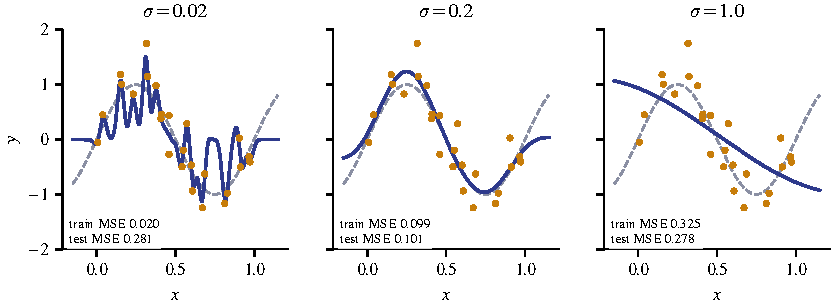
\includegraphics[width=\linewidth]{figures/n10_krr_widths.pdf}
\caption{Kernel ridge regression with a Gaussian kernel and $\lambda = 0.1$ on 25 noisy samples (dots) of
$\sin 2\pi x$ (dashed), for three widths, fitted without centring the targets. Errors are mean squared errors, the
test error on 2000 new samples; the noise variance is 0.09, the smallest test error that any model can reach on average. A narrow kernel
follows the noise and falls back to zero between the points; a wide kernel is too stiff to follow the sine.}
\label{fig:krr}
\end{figure}

Figure~\ref{fig:krr} shows the width at work in regression. With $\sigma = 0.02$ the training mean squared error is small (0.020) but
the test error is 0.281; $\sigma = 0.2$ gives a test error of 0.101, close to the noise level 0.09; $\sigma = 1$ underfits
(training 0.325, test 0.278). The width plays the role of the Parzen bandwidth (Note~5, Section~3) and $\lambda$ that of
the ridge penalty (Note~8, Section~4); together they set the capacity (Note~4, Section~5).

\section{Kernel support vector machines}\label{sec:ksvm}

The SVM of Note~9, Section~5, chooses the maximum-margin hyperplane, and its dual problem (derived there from the
Lagrangian, with the box $0 \le \alpha_i \le C$ of the soft margin) touches the data only through dot products $\x_i\T\x_j$.
In feature space each of them becomes $k(\x_i, \x_j)$, which gives the \emph{kernel SVM}~\cite{boser1992,cortes1995}:
\begin{equation}\label{eq:dual}
  \max_{\valpha}\ \sum_{i=1}^n \alpha_i - \frac12\sum_{i,j=1}^n \alpha_i\alpha_j t_it_j\, k(\x_i, \x_j)
  \quad\text{subject to}\quad 0 \le \alpha_i \le C, \quad \sum_{i=1}^n \alpha_i t_i = 0,
\end{equation}
with $C = \infty$ for the hard margin. Since $K$ is PSD the objective is concave, so every local maximum is global (the
maximiser is unique when $K$ is positive definite). The decision function is
\begin{equation}\label{eq:svmdec}
  g(\x) = \sum_{i=1}^n \alpha_i t_i\, k(\x_i, \x) + b
\end{equation}
(unlike in \eqref{eq:kscore}, here $g$ includes the bias).

\paragraph{Support vectors} At the optimum the Karush--Kuhn--Tucker conditions give three implications: $t_ig(\x_i) > 1$
(beyond the margin) $\Rightarrow \alpha_i = 0$; $0 < \alpha_i < C \Rightarrow t_ig(\x_i) = 1$ (exactly on the margin);
$t_ig(\x_i) < 1$ (inside the margin or misclassified) $\Rightarrow \alpha_i = C$. Note~9 derived the hard-margin
condition $\alpha_i[t_ig(\x_i) - 1] = 0$; for the soft margin, each slack $\xi_i \ge 0$ (at the optimum $\xi_i =
\max(0, 1 - t_ig(\x_i))$) has its own multiplier $\mu_i \ge 0$. Setting the derivative of the Lagrangian with respect to
$\xi_i$ to zero gives $\alpha_i + \mu_i = C$, and complementary slackness gives $\alpha_i[t_ig(\x_i) - 1 + \xi_i] = 0$
and $\mu_i\xi_i = 0$. A point inside the margin has $\xi_i > 0$, so $\mu_i = 0$ and $\alpha_i = C$; a point strictly
beyond it has $\xi_i = 0$ and $t_ig(\x_i) - 1 > 0$, so $\alpha_i = 0$; and $0 < \alpha_i < C$ means $\mu_i > 0$, hence
$\xi_i = 0$ and $t_ig(\x_i) = 1$. Points with $t_ig(\x_i) = 1$ may have any
$\alpha_i$ in $[0, C]$. Only points with $\alpha_i > 0$, the \emph{support vectors}, appear in \eqref{eq:svmdec}; the
others could be deleted without changing the classifier. The bias follows from any support vector $s$ with
$0 < \alpha_s < C$: $b = t_s - \sum_i \alpha_i t_i k(\x_i, \x_s)$ (in practice, averaged over all of them). In
Figure~\ref{fig:kwidths} the good classifiers keep about 40 of the 200 points; the overfitting narrow kernel keeps 158 --- many support vectors is a warning sign.

\begin{worked}{8. The kernel SVM on XOR}
Return to the four XOR points and $k = (1 + \x\T\z)^2$, with $K = 8I + \vect{1}\vect{1}\T$ and $\vect{t} = (1, 1, -1,
-1)$ (hard margin, $C = \infty$). Because $K_{ij} = 8\delta_{ij} + 1$ and $t_i^2 = 1$, the double sum in
\eqref{eq:dual} splits into two simple pieces:
\[
  \sum_{i,j}\alpha_i\alpha_jt_it_jK_{ij} = 8\sum_i \alpha_i^2 + \Big(\sum_i \alpha_it_i\Big)^2 ,
\]
and the constraint $\sum_i\alpha_it_i = 0$ removes the second. On the feasible set the dual objective is therefore
\[
  \sum_i \alpha_i - 4\sum_i \alpha_i^2 = \sum_i \big(\alpha_i - 4\alpha_i^2\big) ,
\]
a sum of separate parabolas. Each term is largest where its derivative $1 - 8\alpha_i$ vanishes, at $\alpha_i = 1/8$,
and $\valpha = \frac18(1, 1, 1, 1)$ also satisfies $\sum_i\alpha_it_i = \frac18(1 + 1 - 1 - 1) = 0$. It maximises every
term at once, so it is the optimum. The bias follows from point~1, a support vector with $0 < \alpha_1 < C$:
\[
  b = t_1 - \sum_i \alpha_it_iK_{i1} = 1 - \tfrac18(9 + 1 - 1 - 1) = 0 ,
\]
and \eqref{eq:svmdec} gives
\[
  g(\x) = \tfrac18 \cdot 8\,x_1x_2 = x_1x_2 ,
\]
using the sum computed in Worked example~4. Every point has $t_ig(\x_i) = 1$: all four are support vectors, on the
margin. In feature space $\norm{\w}^2 = \sum_{i,j}\alpha_i\alpha_jt_it_jK_{ij} = 32/64 = \frac12$, so the geometric
margin is $1/\norm{\w} = \sqrt2$ --- the margin $\gamma$ used in the mistake bound of Worked example~4. The perceptron's
$8x_1x_2$ and the SVM's $x_1x_2$ have the same boundary here only because of the symmetry; in general the perceptron
stops at any separator, the SVM at the one of largest margin.
\end{worked}

\paragraph{Training by dual coordinate ascent} Absorb the bias into the kernel, $\tilde k = k + 1$ (``A bias for free'').
The equality constraint $\sum_i\alpha_it_i = 0$, which came from the derivative with respect to $b$, then disappears and
each $\alpha_i$ can be improved on its own, subject only to $0 \le \alpha_i \le C$. The dual objective is now
\[
  Q(\valpha) = \sum_i \alpha_i - \frac12\sum_{i,j}\alpha_i\alpha_jt_it_j\tilde K_{ij} ,
  \qquad \text{with scores } g_i = \sum_j \alpha_j t_j \tilde K_{ij} .
\]
Change only $\alpha_i$, to $\alpha_i + \delta$. The linear sum grows by $\delta$; in the double sum only the terms with $i$ as one (or both) of the indices change, the
part linear in $\delta$ is $2\delta\,t_i\sum_j\alpha_jt_j\tilde K_{ij} = 2\delta\,t_ig_i$ (the factor 2 because $i$ can be
the first or the second index), and the part quadratic in $\delta$, from the term $(i, i)$, is $\delta^2 t_i^2\tilde K_{ii}
= \delta^2\tilde K_{ii}$. Hence
\[
  Q(\valpha + \delta\,\vect{e}_i) - Q(\valpha) = \delta\,(1 - t_ig_i) - \tfrac12\delta^2\,\tilde K_{ii} ,
\]
a downward parabola in $\delta$ (its first and second derivatives at $\delta = 0$ are $\partial Q/\partial\alpha_i =
1 - t_ig_i$ and $-\tilde K_{ii}$) with its top at $\delta = (1 - t_ig_i)/\tilde K_{ii}$. Move there, clip to $[0, C]$,
update all scores, and sweep repeatedly (Algorithm~\ref{alg:ksvm}). Unlike for the perceptron, absorbing the bias
slightly changes the problem: the bias is now the weight of a constant feature and is penalised like the other weights,
so the SVM minimises $\frac12(\norm{\w}^2 + b^2)$ instead of $\frac12\norm{\w}^2$. The two solutions usually differ only
a little, and they coincide when the free-bias optimum has $b = 0$, as in Worked example~8. This scheme is a simplified
relative of SMO~\cite{platt1998}, which keeps a separate bias and therefore changes two multipliers at a time.

\begin{algorithm}[htbp]
\caption{Kernel SVM: training by dual coordinate ascent, and prediction}\label{alg:ksvm}
\begin{algorithmic}[1]
\Require training set $\{(\x_i, t_i)\}_{i=1}^n$, kernel $k$, $C > 0$, number of sweeps $E$
\Function{KernelSVMFit}{$\{(\x_i, t_i)\}$; $k, C, E$}
  \State $\tilde K \gets \textsc{Gram}(X; k) + \vect{1}\vect{1}\T$ \Comment{bias absorbed, $O(n^2 d)$}
  \State $\valpha \gets \vect{0}$; \ $\vect{g} \gets \vect{0}$ \Comment{$g_i = \sum_j \alpha_j t_j \tilde K_{ij}$}
  \For{sweep $= 1, \dots, E$}
    \For{$i = 1, \dots, n$ in random order}
      \State $a \gets \min\!\big(C, \max(0,\ \alpha_i + (1 - t_ig_i)/\tilde K_{ii})\big)$ \Comment{$O(1)$}
      \State $\vect{g} \gets \vect{g} + (a - \alpha_i)\,t_i\,\tilde K_{:,i}$; \ $\alpha_i \gets a$ \Comment{$O(n)$}
    \EndFor
  \EndFor
  \State \Return $\valpha$ \Comment{support vectors: $\alpha_i > 0$}
\EndFunction
\Function{KernelSVMPredict}{$\x$; $\{(\x_s, t_s, \alpha_s)\}_{\alpha_s > 0}$, $k$}
  \State \Return $\operatorname{sign}\big(\sum_{s} \alpha_s t_s\, [k(\x_s, \x) + 1]\big)$ \Comment{$O(n_{\mathrm{SV}}\, d)$}
\EndFunction
\end{algorithmic}
\end{algorithm}

\begin{runtime}{kernel SVM}
\emph{Training}: $O(n^2 d)$ for the Gram matrix, then $O(n)$ per coordinate update and $O(En^2)$ for $E$ sweeps.
Generic quadratic-programming solvers cost $O(n^3)$; SMO, used in the LIBSVM library, needs between $O(n^2)$ and
$O(n^3)$ kernel evaluations ($O(n^2 d)$ to $O(n^3 d)$ time), depending on $C$ and on the data. \emph{Memory}: $O(n^2)$, or a cache of the most used rows of $K$.
\emph{Prediction}: $O(n_{\mathrm{SV}}\,d)$ per query.
\end{runtime}

\begin{worked}{9. Dual coordinate ascent on XOR, by hand}
Run Algorithm~\ref{alg:ksvm} on the XOR data of Worked example~8, with $C$ so large that it never clips and the fixed
order $1, 2, 3, 4$. With the bias absorbed, $\tilde K = K + \vect{1}\vect{1}\T$ has $10$ on the diagonal and $2$
elsewhere, so each update is $\alpha_i \gets \alpha_i + (1 - t_ig_i)/10$, after which the score vector changes by
$(\text{change of }\alpha_i)\,t_i$ times column $i$ of $\tilde K$. The first sweep, starting from $\valpha = \vect{0}$,
$\vect{g} = \vect{0}$:
\begin{center}\small
\begin{tabular}{@{}cccl@{}}
\toprule
$i$ & $t_ig_i$ before & new $\alpha_i$ & $(t_1g_1, t_2g_2, t_3g_3, t_4g_4)$ after \\
\midrule
1 & $0$ & $0.1$ & $(1,\ 0.2,\ -0.2,\ -0.2)$ \\
2 & $0.2$ & $0.08$ & $(1.16,\ 1,\ -0.36,\ -0.36)$ \\
3 & $-0.36$ & $0.136$ & $(0.888,\ 0.728,\ 1,\ -0.088)$ \\
4 & $-0.088$ & $0.1088$ & $(0.670,\ 0.510,\ 1.218,\ 1)$ \\
\bottomrule
\end{tabular}
\end{center}
Each update puts its own point exactly on the margin ($t_ig_i = 1$), but moves the others: after sweep~1,
$\valpha = (0.1, 0.08, 0.136, 0.1088)$. After sweep~2, $\valpha = (0.133, 0.122, 0.129, 0.125)$ and the margins are
$(1.065, 0.981, 1.033, 1)$; after sweep~5 every $\alpha_i$ agrees with $1/8$ to four decimals and every $t_ig_i$ lies within
$0.0003$ of $1$. The iteration has found the analytic optimum of Worked example~8. Absorbing the bias did not change it, because
there $\sum_i\alpha_it_i = 0$: the absorbed bias $b = \sum_i\alpha_it_i$ is zero at the optimum, as was the free one.
\end{worked}

\section{The kernel family}\label{sec:family}

\paragraph{Kernelisable algorithms} Many linear algorithms can be written with dot products only, and each has a kernel
version. They differ in what the coefficients mean, whether most of them vanish, and what training costs (all start with
the $O(n^2 d)$ Gram matrix; $T$ is a number of passes or iterations, $E$ a number of sweeps):
\begin{center}\small
\begin{tabular}{@{}L{0.25\linewidth}L{0.31\linewidth}L{0.11\linewidth}L{0.23\linewidth}@{}}
\toprule
algorithm & coefficient of example $i$ & sparse? & training beyond $K$ \\
\midrule
perceptron (Section~\ref{sec:trick}) & number of mistakes on $i$ & yes & $O(Tn^2)$ \\
SVM (Section~\ref{sec:ksvm}) & Lagrange multiplier of the margin constraint & yes & $O(En^2)$ to $O(n^3)$ \\
ridge regression (Section~\ref{sec:krr}) & residual of $i$, divided by $\lambda$ & no & $O(n^3)$ \\
logistic regression (Algorithm~\ref{alg:klr}) & weight $\beta_i$ in $g = \sum_i \beta_i k(\x_i, \cdot)$ & no & $O(Tn^2)$ by gradient descent \\
support vector regression & multiplier of the $\varepsilon$-tube constraint & yes & as the SVM \\
Gaussian process & as ridge, $\lambda = $ noise variance & no & $O(n^3)$; error bar $O(n^2)$ per query \\
kernel PCA & component of an eigenvector of centred $K$ & no & $O(n^3)$ eigendecomposition \\
\bottomrule
\end{tabular}
\end{center}
Plain (unregularised) least squares is also in the family: it is the limit $\lambda \to 0$ of kernel ridge regression,
$K\valpha = \y$, which for an invertible $K$ --- the Gaussian kernel on distinct points --- interpolates the training data
(Section~\ref{sec:krr}, ``What $\lambda$ does''); that is why $\lambda > 0$ is used in practice.

\emph{Kernel logistic regression} uses $0/1$ labels as in Note~9, Section~4, written here $y_i = (1 + t_i)/2 \in \{0, 1\}$, the score
$g(\x) = \sum_i \beta_i k(\x_i, \x)$ (a bias absorbed as in ``A bias for free'') and the probability $\sigma(g)$, with
$\sigma(a) = 1/(1 + e^{-a})$. On the training points the scores are $\vect{g} = K\vect{\beta}$, and it minimises the
cross-entropy plus the penalty $\lambda\vect{\beta}\T K\vect{\beta}$, which equals $\lambda\norm{\w}^2$ for
$\w = \sum_i\beta_i\phi(\x_i)$:
\[
  J(\vect{\beta}) = -\sum_i \big[y_i\log\sigma(g_i) + (1 - y_i)\log(1 - \sigma(g_i))\big] + \lambda\vect{\beta}\T K\vect{\beta} ,
  \qquad
  \nabla J = K\big(\sigma(K\vect{\beta}) - \y\big) + 2\lambda K\vect{\beta} .
\]
The gradient follows from the chain rule: the cross-entropy has derivative $\sigma(g_i) - y_i$ with respect to $g_i$
(Note~9, Section~4), and $\partial g_i/\partial\beta_j = K_{ij}$. There is no closed form, so the minimiser is found by
gradient descent (Note~7), Algorithm~\ref{alg:klr}. It gives probabilities but, unlike the SVM, keeps every training
point.

\begin{algorithm}[htbp]
\caption{Kernel logistic regression by gradient descent}\label{alg:klr}
\begin{algorithmic}[1]
\Require training set $\{(\x_i, t_i)\}_{i=1}^n$, kernel $k$, $\lambda > 0$, step size $\eta$, number of iterations $T$
\Function{KLRFit}{$\{(\x_i, t_i)\}$; $k, \lambda, \eta, T$}
  \State $K \gets \textsc{Gram}(X; k) + \vect{1}\vect{1}\T$; \ $y_i \gets (1 + t_i)/2$ \Comment{bias absorbed, $O(n^2 d)$}
  \State $\vect{\beta} \gets \vect{0}$
  \For{iteration $= 1, \dots, T$}
    \State $\vect{r} \gets \sigma(K\vect{\beta}) - \y$ \Comment{residuals of the probabilities, $O(n^2)$}
    \State $\vect{\beta} \gets \vect{\beta} - \eta\, K(\vect{r} + 2\lambda\vect{\beta})$ \Comment{gradient step, $O(n^2)$}
  \EndFor
  \State \Return $\vect{\beta}$
\EndFunction
\Function{KLRPredict}{$\x$; $\{(\x_i, \beta_i)\}$, $k$}
  \State \Return $P(t = +1 \mid \x) = \sigma\big(\sum_i \beta_i\,[k(\x_i, \x) + 1]\big)$ \Comment{$O(nd)$}
\EndFunction
\end{algorithmic}
\end{algorithm}

\begin{runtime}{kernel logistic regression}
\emph{Training}: $O(n^2 d)$ for the Gram matrix, then two matrix--vector products with $K$, $O(n^2)$, per iteration:
$O(n^2 d + Tn^2)$ in total (Newton's method would converge in fewer iterations but costs $O(n^3)$ per step).
\emph{Memory}: $O(n^2)$ for $K$. \emph{Prediction}: $O(nd)$ per query, since all $\beta_i$ are non-zero in general.
\end{runtime}

The remaining rows of the table are mentioned for orientation and are not developed here. Support vector regression ignores errors smaller than
$\varepsilon$, which is what makes it sparse. A \emph{Gaussian process}~\cite{rasmussen2006} is the Bayesian version of
ridge regression (Note~8, Section~6): its predictive mean is exactly \eqref{eq:krrpred} with $\lambda$ equal to the noise
variance, and it adds an error bar; in geostatistics the same method is called kriging. Kernel PCA diagonalises the
centred Gram matrix and finds non-linear directions of variation~\cite{scholkopf1998}; projecting a new point on $q$
components costs $O(nd + nq)$. Algorithms that look at single coordinates rather than dot products, such as decision trees
(Note~3, Section~4), do not kernelise.

\paragraph{Two meanings of ``kernel''} Note~5, Section~3, used a kernel as a \emph{smoothing window} --- written
$K(\x_i, \x)$ there, $w(\x_i, \x)$ here to avoid a clash with the Gram matrix: a non-negative weight, decreasing with
distance, used in a weighted average $\sum_i w\,y_i / \sum_i w$ with no training at all. This note's kernels are
\emph{Mercer kernels}: dot products in a feature space, with PSD Gram matrices, whose coefficients $\alpha_i$ are
learned. The requirements differ:
\begin{center}\small
\begin{tabular}{@{}L{0.17\linewidth}L{0.37\linewidth}L{0.37\linewidth}@{}}
\toprule
& smoothing kernel (Note~5) & Mercer kernel (this note) \\
\midrule
requirement & non-negative, peaked at $\x = \z$, decreasing with distance; integrates to 1 for density estimation &
symmetric, every Gram matrix PSD \\
prediction & $\sum_i w(\x_i, \x)\,y_i \big/ \sum_i w(\x_i, \x)$ & $\sum_i \alpha_i\, k(\x_i, \x)$, $\valpha$ fitted \\
training & none & solve for $\valpha$ \\
examples & Gaussian, box window, Epanechnikov & Gaussian, polynomial, linear, Laplacian \\
\bottomrule
\end{tabular}
\end{center}
The Gaussian is both, which is why the word is shared. The other entries are not interchangeable. The polynomial kernel
$(1 + \x\T\z)^3$ is a valid Mercer kernel but a useless smoothing window: it grows with distance and can be negative. The box
window $\ind{|x - z| < 1}$ is a fine smoothing window but not a Mercer kernel: on the points $0, 0.6, 1.2$ its Gram matrix is
\[
  \begin{pmatrix} 1 & 1 & 0 \\ 1 & 1 & 1 \\ 0 & 1 & 1 \end{pmatrix}, \qquad \vect{c} = (1, -1, 1):\ \
  \vect{c}\T K\vect{c} = 3 - 2 - 2 + 0 = -1 < 0 ,
\]
with eigenvalues $1 - \sqrt2$, $1$ and $1 + \sqrt2$. Note also that Section~\ref{sec:krr} links the two worlds: for large
$\lambda$, kernel ridge regression becomes a Parzen-like weighted sum of the targets.

\section{Running time and scaling to many examples}\label{sec:cost}

Table~\ref{tab:cost} collects the costs, with $n$ examples in $d$ dimensions, $D$ explicit features, $T$ passes or $E$
sweeps, and $n_{\mathrm{SV}}$ support vectors.

\begin{table}[h]
\centering\small
\caption{Costs of explicit and kernel methods. Kernel evaluations are assumed to cost $O(d)$; $D$ is the number of
features of whichever explicit map is used (polynomial or random Fourier).}
\label{tab:cost}
\begin{tabular}{@{}L{0.33\linewidth}L{0.22\linewidth}L{0.15\linewidth}L{0.19\linewidth}@{}}
\toprule
method & training time & memory & prediction / query \\
\midrule
explicit map + perceptron or GD & $O(nD + TnD)$ & $O(nD)$ & $O(D)$ \\
explicit map + ridge (primal) & $O(nD^2 + D^3)$ & $O(nD + D^2)$ & $O(D)$ \\
Gram matrix & $O(n^2 d)$ & $O(n^2)$ & --- \\
kernel perceptron & $O(n^2 d + Tn^2)$ & $O(n^2)$ & $O(Md)$, $M \le n$ \\
kernel ridge regression & $O(n^2 d + n^3)$ & $O(n^2)$ & $O(nd)$ \\
kernel SVM & $O(n^2 d + En^2)$; SMO $O(n^2 d)$ to $O(n^3 d)$ & $O(n^2)$ or cache & $O(n_{\mathrm{SV}}\,d)$ \\
kernel logistic regression & $O(n^2 d + Tn^2)$ & $O(n^2)$ & $O(nd)$ \\
random Fourier features $\hat\phi$ + ridge & $O(nDd + nD^2 + D^3)$ & $O(nD)$ & $O(Dd)$ \\
\bottomrule
\end{tabular}
\end{table}

\paragraph{Which is cheaper} The explicit route pays for the dimension $D$ of the feature space; the kernel route pays
for the number of examples, through the $n \times n$ Gram matrix. Kernels win when $D$ is huge or infinite and $n$ is
moderate --- up to some $10^4$ to $10^5$ examples, a regime common in physics, where each example may be an expensive
simulation or measurement. Explicit or learned features win when $n$ is in the millions, where an $n \times n$ matrix can
neither be stored nor factorised.

\paragraph{Random Fourier features} For large $n$ one can return to an explicit map that \emph{approximates} a given
kernel with a modest number $D$ of features~\cite{rahimi2007} ($D$ now counts random features). For the Gaussian kernel
the construction takes a few lines. Let $\vect{\omega} \sim \Normal(\vect{0}, \sigma^{-2}I)$ and $\tau \sim
\mathrm{Uniform}[0, 2\pi]$ (a random phase). For a fixed vector $\vect{u}$, $Y = \vect{\omega}\T\vect{u}$ is a
one-dimensional centred Gaussian with variance $\rho^2 = \norm{\vect{u}}^2/\sigma^2$, and a centred Gaussian has
$\E[\cos Y] = \exp(-\rho^2/2)$. To see this, write $\cos Y$ as the real part of $e^{iY}$ and complete the square in the
exponent, $iy - y^2/2\rho^2 = -(y - i\rho^2)^2/2\rho^2 - \rho^2/2$:
\[
  \E[e^{iY}] = \frac{1}{\sqrt{2\pi\rho^2}}\int_{-\infty}^{\infty} e^{iy - y^2/2\rho^2}\,dy
  = e^{-\rho^2/2}\,\frac{1}{\sqrt{2\pi\rho^2}}\int_{-\infty}^{\infty} e^{-(y - i\rho^2)^2/2\rho^2}\,dy = e^{-\rho^2/2} ,
\]
because the last integral, a Gaussian shifted parallel to the real axis, still equals $\sqrt{2\pi\rho^2}$. (Without complex
numbers: expand $\cos Y = \sum_m (-1)^mY^{2m}/(2m)!$ and use $\E[Y^{2m}] = (2m - 1)(2m - 3)\cdots 1\cdot \rho^{2m}$, which
gives the series of $e^{-\rho^2/2}$ term by term.) So $\E[\cos(\vect{\omega}\T\vect{u})] = \exp(-\norm{\vect{u}}^2/2\sigma^2)$.
The identity $2\cos A\cos B = \cos(A - B) + \cos(A + B)$ with $A = \vect{\omega}\T\x + \tau$, $B = \vect{\omega}\T\z +
\tau$ then gives
\[
  \E\big[2\cos(\vect{\omega}\T\x + \tau)\cos(\vect{\omega}\T\z + \tau)\big]
  = \E\big[\cos(\vect{\omega}\T(\x - \z))\big] + \underbrace{\E\big[\cos(\vect{\omega}\T(\x + \z) + 2\tau)\big]}_{0}
  = k_\sigma(\x, \z) ,
\]
where the second term averages to zero because $2\tau$ runs uniformly over two whole periods of the cosine. Averaging
over $D$ independent draws $(\vect{\omega}_j, \tau_j)$, the random-feature map $\hat\phi(\x)$ with components
$\hat\phi_j(\x) = \sqrt{2/D}\,\cos(\vect{\omega}_j\T\x + \tau_j)$ satisfies $\hat\phi(\x)\T\hat\phi(\z) \approx
k_\sigma(\x, \z)$. Its root-mean-square error is $\sqrt{(1 - k_\sigma^2 + k_\sigma^4/2)/D}$, writing $k_\sigma$ for
$k_\sigma(\x, \z)$: one term $2\cos A\cos B$ has mean $k_\sigma$ and mean square $\E[\cos^2(\vect{\omega}\T(\x - \z))] +
\E[\cos^2(\vect{\omega}\T(\x + \z) + 2\tau)] = \frac12(1 + k_\sigma^4) + \frac12$ (the cross term averages to zero over
$\tau$), hence variance $1 - k_\sigma^2 + k_\sigma^4/2$, and averaging $D$ independent terms divides the variance by $D$.
For $\x = (1, 0)$, $\z = (0, 1)$ and $\sigma = 1$, where $k_\sigma = e^{-1} = 0.368$, this is $0.93/\sqrt D$: $0.30$,
$0.093$, $0.030$ and $0.009$ for $D = 10$, $100$, $1000$ and $10\,000$ (a simulation with 1000 draws agrees to within
3\%). A linear method on $\hat\phi(\x)$ then costs time linear in $n$. The random draw is made once and reused: training
and test points must be mapped with the same $\Omega$ and $\vect{\tau}$ (Algorithm~\ref{alg:rff}). A second remedy, the
Nyström method, approximates $K$ from $m$ randomly chosen columns at cost $O(nmd + nm^2)$~\cite{williams2001}; like
the other methods mentioned only for orientation, it is not developed here.

\begin{algorithm}[htbp]
\caption{Random Fourier features for the Gaussian kernel}\label{alg:rff}
\begin{algorithmic}[1]
\Require input dimension $d$, width $\sigma$, number of features $D$
\Function{RFFDraw}{$d$; $\sigma, D$} \Comment{called once, before training}
  \State draw $\Omega \in \R^{D \times d}$ with entries $\Normal(0, \sigma^{-2})$ and $\vect{\tau} \in [0, 2\pi]^D$ uniformly
  \State \Return $(\Omega, \vect{\tau})$
\EndFunction
\Function{RFFMap}{$X$; $\Omega, \vect{\tau}$} \Comment{same $(\Omega, \vect{\tau})$ for training and test data}
  \State $\hat\Phi \gets \sqrt{2/D}\, \cos\big(X\Omega\T + \vect{1}\vect{\tau}\T\big)$ \Comment{$n \times D$, rows $\hat\phi(\x_i)\T$, $O(nDd)$}
  \State \Return $\hat\Phi$ \Comment{then fit ridge or a linear classifier on $\hat\Phi$}
\EndFunction
\end{algorithmic}
\end{algorithm}

\begin{runtime}{random Fourier features}
\emph{Features}: $O(nDd)$ time and $O(nD)$ memory. \emph{Ridge on top}: $O(nD^2 + D^3)$, linear in $n$; with $D = 10^3$
this handles millions of examples. \emph{Prediction}: $O(Dd)$ per query, independent of $n$. The price is an approximation
error of order $1/\sqrt D$ in each kernel value.
\end{runtime}

\begin{modern}{wide neural networks are kernel machines}
Random features are a neural network whose first layer is frozen at random values and whose last layer is trained.
Note~4, Section~8, showed double descent for exactly such a model. At $D \approx n$, the interpolation threshold, the
minimum-norm solution sits at the double-descent peak; only as $D$ grows far beyond $n$ ($D \to \infty$) does it approach the minimum-norm interpolant
(kernel regression with $\lambda \to 0$) of the kernel that the features approximate~\cite{belkin2019} --- for random ReLU
features, the arc-cosine kernel~\cite{cho2009}. Jacot, Gabriel and Hongler showed that something similar holds for the
\emph{whole} network: with the standard (NTK) scaling of the weights, as every layer becomes infinitely wide, the
\emph{neural tangent kernel} $\Theta(\x, \z) = \nabla_{\vect{\theta}} f(\x)\T\nabla_{\vect{\theta}} f(\z)$ becomes
deterministic and stays constant during training, so gradient descent on the network is kernel gradient descent with a
fixed kernel~\cite{jacot2018}. In this regime wide networks are kernel methods; conversely, kernel machines that
interpolate their training data show the same surprisingly good generalisation as over-parametrised
networks~\cite{belkin2018}. Practical networks are not in this limit: their features move during training, the third
route of Section~\ref{sec:explicit}, and this feature learning is a leading explanation of why they beat fixed kernels on
images and text. Week~5 starts there.
\end{modern}

\begin{physics}{kernel regression of potential-energy surfaces}
Quantum-mechanical calculations of the energy and forces of a configuration of atoms are accurate but slow; molecular
dynamics needs millions of them. Bart\'ok, Payne, Kondor and Cs\'anyi introduced \emph{Gaussian approximation potentials}
(GAP)~\cite{bartok2010}: the total energy is written as a sum of local atomic energies, each a Gaussian-process (that is,
kernel) regression on a descriptor of the atom's neighbourhood that is invariant under rotations, translations and
permutations of identical atoms. Such potentials approach quantum-mechanical accuracy at a small fraction of the
cost. Rupp, Tkatchenko, M\"uller and von Lilienfeld similarly used kernel
ridge regression on a matrix of Coulomb repulsions between nuclei to predict the atomisation energies of several thousand
small organic molecules~\cite{rupp2012}. In both cases the physics enters through the kernel: what does it mean for two
atomic environments to be similar?
\end{physics}

\begin{keyidea}[Summary]
A fixed non-linear feature map $\phi$ turns any linear method into a non-linear one; explicit polynomial maps have
$\binom{d+p}{p}$ features and quickly become too large. Algorithms that use the data only through dot products --- the
perceptron, ridge regression, the SVM, logistic regression, PCA --- can instead be written with coefficients
$\alpha_i$, one per training example, and a kernel $k(\x, \z) = \phi(\x)\T\phi(\z)$ that is cheap to evaluate even when
$\phi$ is infinite-dimensional, as for the Gaussian kernel. A function is a valid kernel exactly when its Gram matrices are
symmetric positive semi-definite; sums, positive multiples and products of kernels are kernels. The kernel perceptron
counts mistakes, kernel ridge regression solves $(K + \lambda I)\valpha = \y$, and the kernel SVM keeps only its support
vectors. The kernel width and the regularisation constant set the capacity and are chosen by validation. The price is an
$n \times n$ Gram matrix: $O(n^2)$ memory and up to $O(n^3)$ time, which random features or learned features avoid when
$n$ is large.
\end{keyidea}

\begin{questions}
\begin{conceptual}
\item Explain how a linear classifier trained on $\phi(\x)$ can have a curved decision boundary in the input space. For the
  quadratic map $\phi(x_1, x_2) = (x_1, x_2, x_1^2, x_1x_2, x_2^2)$, which shapes of boundary are possible?
\item In the centred coordinates $s_j = 2x_j - 1$ of Section~\ref{sec:why}, the class of each XOR point is the sign of
  $s_1s_2$. Explain why adding this single feature makes the points linearly separable, and describe the resulting
  boundary in the original $(x_1, x_2)$ plane.
\item Name the three routes to a non-linear feature map discussed in Section~\ref{sec:explicit}. Give one advantage and
  one disadvantage of each.
\item True or false, with a justification: ``The kernel trick is a fast method for computing $\phi(\x)$.''
\item Explain in words why adding to $\w$ a component orthogonal to all the $\phi(\x_i)$ can only increase a
  ridge-regularised objective. What does this imply about how many numbers are needed to describe the solution when the
  feature space is infinite-dimensional?
\item In the kernel perceptron, what does $\alpha_i$ count? What does $\alpha_i = 0$ say about example $i$, and why do
  such examples cost nothing at prediction time?
\item A student trains a linear perceptron on the raw inputs, obtains $\w = \sum_i \alpha_it_i\x_i$, and then uses
  $\phi(\w)$ as the weight vector in feature space. Explain why this is not the kernel perceptron.
\item Describe what happens to the Gram matrix and to the decision boundary of a Gaussian-kernel classifier as
  $\sigma \to 0$ and as $\sigma \to \infty$. Which regime overfits? Relate your answer to Figure~\ref{fig:kwidths}.
\item Why must every Gram matrix of a valid kernel be positive semi-definite? Explain the argument in terms of the length of
  a vector in feature space.
\item Without expanding any feature map, decide which of these are valid kernels on $\R^d$ and justify each answer with a rule
  of Section~\ref{sec:mercer} or a counter-example: (a)~$3\,\x\T\z$; (b)~$-\x\T\z$; (c)~$(\x\T\z)^2 + 1$;
  (d)~$\norm{\x - \z}^2$; (e)~$k_\sigma(\x, \z)\,(1 + \x\T\z)^2$.
\item In kernel ridge regression, what happens to the fit as $\lambda \to 0$ and as $\lambda \to \infty$? Why does the
  prediction of a Gaussian-kernel model return to zero far from the data, and why does this make centring the targets
  important?
\item Which training points are support vectors of a kernel SVM? Why does the prediction cost depend on their number, and
  what might a very large number of support vectors indicate?
\item Compare the kernel perceptron, kernel ridge regression and the kernel SVM with respect to how many coefficients
  $\alpha_i$ are non-zero after training.
\item The Gaussian function appears in both Note~5 (Parzen windows) and this note. Explain the different roles it plays.
  Give one function that is a good smoothing window but not a Mercer kernel, and one Mercer kernel that is not a useful
  smoothing window.
\item You have $n = 10^6$ examples with $d = 20$ features. Explain why exact kernel ridge regression is impractical, and
  describe two alternatives.
\item For ridge regression with a polynomial kernel, when is the explicit (primal) form cheaper to train than kernel
  ridge regression? Answer in terms of $n$ and $D$.
\item Why should the input features be standardised before a Gaussian kernel is used? Give an example of what goes wrong
  otherwise.
\item True or false, with a justification: ``A kernel method has no hyperparameters, because the kernel is chosen in
  advance.''
\item Random Fourier features are a neural network whose first layer is frozen at random values. What is trained in such
  a model, and what does a practical neural network learn that a fixed-kernel method cannot?
\end{conceptual}

\begin{calculations}
\item How many monomials of degree at most 2 are there in $d = 3$ variables? List them. How many of degree at most 4 in
  $d = 20$ variables?
\item For $\x = (2, -1)$ and $\z = (1, 3)$ compute $(\x\T\z)^2$ directly, and again as $\phi(\x)\T\phi(\z)$ with the
  map $\phi(\x) = (x_1^2, \sqrt2\,x_1x_2, x_2^2)$. Then do the same for $(1 + \x\T\z)^2$ with the six-dimensional map of
  Worked example~3.
\item Run the kernel perceptron (Algorithm~\ref{alg:kperc}) on the one-dimensional data $x = -2, -1, 1, 2$ with labels
  $t = +1, -1, -1, +1$ and the kernel $k(x, z) = (1 + xz)^2$, visiting the points in this order. First compute the
  $4 \times 4$ Gram matrix. Then carry out the first two passes and report $\valpha$ after each. (Continued, the
  algorithm makes no mistake in its fourth pass and stops with $\valpha = (1, 3, 3, 1)$.) Using this final $\valpha$,
  write the decision function $g(x)$ as a polynomial in $x$. Where is the decision boundary? Compare with the explicit
  route of Worked example~2.
\item Show that $\begin{pmatrix} 1 & 2 \\ 2 & 1 \end{pmatrix}$ cannot be the Gram matrix of any kernel by exhibiting a
  vector $\vect{c}$ with $\vect{c}\T K\vect{c} < 0$. Then compute the Gram matrix of the Gaussian kernel with $\sigma = 1$
  on the points $x = 0, 1, 3$ (four decimals) and check that its leading principal minors (the determinants of its
  top-left $1 \times 1$, $2 \times 2$ and $3 \times 3$ sub-matrices) are positive.
\item Kernel ridge regression with two points: $x_1 = 0$, $x_2 = 1$, targets $\y = (1, -1)$, a Gaussian kernel with
  $k(0, 1) = 0.5$, and $\lambda = 0.5$. Compute $\valpha = (K + \lambda I)^{-1}\y$, the fitted values at the two training
  points, and the predictions at $x = 0.5$ and $x = -0.5$, using $k(0, \pm 0.5) = k(1, 0.5) = 0.841$ and
  $k(1, -0.5) = 0.210$.
\item A kernel SVM with $k(x, z) = (1 + xz)^2$ trained on $x = -1, 0, 1$ with labels $t = +1, -1, +1$ returned $\valpha =
  (1, 2, 1)$ and $b = -1$. Check that $\sum_i\alpha_it_i = 0$, write $g(x)$ as a polynomial, evaluate it at $x = 0.5$ and
  $x = 2$, verify that all three points lie on the margin, and find the decision boundary.
\item For the one-dimensional Gaussian kernel $k(x, z) = \exp(-(x - z)^2/2\sigma^2)$, compute $\partial k/\partial x$.
  At which distances $|x - z|$ does the kernel decrease fastest? Interpret $\sigma$ as a length scale.
\item You have $n = 5 \times 10^4$ examples in $d = 100$ dimensions and compare kernel ridge regression with the kernel
  $k(\x, \z) = (1 + \x\T\z)^2$ against primal ridge regression on its $D = \binom{102}{2}$ explicit features (constant
  included). Compute $D$ and estimate (a)~the memory of the Gram matrix in 64-bit floats, (b)~the number of operations to
  compute it ($\approx n^2d$), (c)~the number of operations for the Cholesky factorisation in kernel ridge regression
  ($\approx n^3/3$), (d)~the memory of the explicit features in 64-bit floats, and (e)~the number of operations of the
  primal solution, $\approx nD^2 + D^3$. Which approach would you choose?
\end{calculations}

\begin{derivations}
\item Show that $(1 + \x\T\z)^2 = \phi(\x)\T\phi(\z)$ for $\x, \z \in \R^d$ with an explicit $\phi$, and check that its
  dimension is $\binom{d+2}{2}$. Then prove \eqref{eq:count} by the dummy-variable argument of Section~\ref{sec:explicit}.
\item Prove the push-through identity and use it to derive $\valpha = (K + \lambda I)^{-1}\y$ for kernel ridge regression.
  Show that the fitted values are $K(K + \lambda I)^{-1}\y$, and that the fit interpolates the data as $\lambda \to 0$ when
  $K$ is invertible.
\item Prove that the sum, the positive multiple and the product of two kernels are kernels, by constructing their feature
  maps. Deduce that the Gaussian kernel is valid in any dimension.
\item Starting from the linear SVM dual of Note~9, Section~5, explain which quantities change when the inputs are
  replaced by $\phi(\x_i)$, and obtain \eqref{eq:dual}. Show that keeping a bias in the kernel perceptron is equivalent to
  replacing $k$ by $k + 1$. Then, for the SVM with $\tilde k = k + 1$ and no separate bias, derive the coordinate update of
  Algorithm~\ref{alg:ksvm} from the first and second derivatives of the dual objective with respect to $\alpha_i$.
\end{derivations}

\begin{programming}
\item Implement Algorithms~\ref{alg:gram} and~\ref{alg:kperc} in numpy and run the kernel perceptron on noisy two-moons
  data with a cubic polynomial kernel and Gaussian kernels of several widths. Plot the decision regions, and report the
  number of mistakes and the number of non-zero $\alpha_i$. What happens when the data are not separable in feature space?
\item Implement kernel ridge regression (Algorithm~\ref{alg:krr}) and reproduce Figure~\ref{fig:krr} (the figure was
  fitted without centring the targets, so with centring your curves will differ slightly, mostly near the ends). Choose $\sigma$ and
  $\lambda$ by 5-fold cross-validation and compare the result with polynomial ridge regression (Note~8) of the best degree.
\item Implement random Fourier features (Algorithm~\ref{alg:rff}). (a)~Plot the error of $\hat\phi(\x)\T\hat\phi(\z)$ as an
  approximation of $k_\sigma(\x, \z)$ against $D$ on log--log axes and confirm the $1/\sqrt D$ slope. (b)~For $n$ from
  $10^3$ to $2 \times 10^4$, time exact kernel ridge regression and ridge regression on $D = 500$ random features, and
  compare their test errors.
\end{programming}
\end{questions}

\paragraph{Further reading} Bishop~\cite{bishop2006}, chapters~6 and~7; Hastie, Tibshirani and Friedman~\cite{hastie2009},
sections~5.8 and~12.3; Murphy~\cite{murphy2022}, chapter~17; Sch\"olkopf and Smola~\cite{scholkopf2002} for the theory of
kernels; Rasmussen and Williams~\cite{rasmussen2006} for Gaussian processes, the probabilistic reading of kernel ridge
regression.

\begin{thebibliography}{99}\small
\bibitem{aizerman1964} M.~A. Aizerman, E.~M. Braverman and L.~I. Rozonoer, Theoretical foundations of the potential function method in pattern recognition learning, \emph{Autom.\ Remote Control} 25, 821--837 (1964).
\bibitem{bartok2010} A.~P. Bart\'ok, M.~C. Payne, R.~Kondor and G.~Cs\'anyi, Gaussian approximation potentials: the accuracy of quantum mechanics, without the electrons, \emph{Phys.\ Rev.\ Lett.}\ 104, 136403 (2010).
\bibitem{belkin2018} M.~Belkin, S.~Ma and S.~Mandal, To understand deep learning we need to understand kernel learning, \emph{ICML} (2018).
\bibitem{belkin2019} M.~Belkin, D.~Hsu, S.~Ma and S.~Mandal, Reconciling modern machine-learning practice and the classical bias--variance trade-off, \emph{Proc.\ Natl.\ Acad.\ Sci.\ USA} 116, 15849--15854 (2019).
\bibitem{bishop2006} C.~M. Bishop, \emph{Pattern Recognition and Machine Learning}, Springer (2006).
\bibitem{boser1992} B.~E. Boser, I.~M. Guyon and V.~N. Vapnik, A training algorithm for optimal margin classifiers, \emph{Proc.\ 5th Annual Workshop on Computational Learning Theory (COLT)}, 144--152 (1992).
\bibitem{cho2009} Y.~Cho and L.~K. Saul, Kernel methods for deep learning, \emph{NeurIPS} (2009).
\bibitem{cortes1995} C.~Cortes and V.~Vapnik, Support-vector networks, \emph{Mach.\ Learn.}\ 20, 273--297 (1995).
\bibitem{freund1999} Y.~Freund and R.~E. Schapire, Large margin classification using the perceptron algorithm, \emph{Mach.\ Learn.}\ 37, 277--296 (1999).
\bibitem{hastie2009} T.~Hastie, R.~Tibshirani and J.~Friedman, \emph{The Elements of Statistical Learning}, 2nd ed., Springer (2009).
\bibitem{jacot2018} A.~Jacot, F.~Gabriel and C.~Hongler, Neural tangent kernel: convergence and generalization in neural networks, \emph{NeurIPS} (2018).
\bibitem{kimeldorf1971} G.~Kimeldorf and G.~Wahba, Some results on Tchebycheffian spline functions, \emph{J.\ Math.\ Anal.\ Appl.}\ 33, 82--95 (1971).
\bibitem{mercer1909} J.~Mercer, Functions of positive and negative type, and their connection with the theory of integral equations, \emph{Phil.\ Trans.\ R.\ Soc.\ Lond.\ A} 209, 415--446 (1909).
\bibitem{murphy2022} K.~P. Murphy, \emph{Probabilistic Machine Learning: An Introduction}, MIT Press (2022).
\bibitem{platt1998} J.~C. Platt, Sequential minimal optimization: a fast algorithm for training support vector machines, Microsoft Research Technical Report MSR-TR-98-14 (1998).
\bibitem{rahimi2007} A.~Rahimi and B.~Recht, Random features for large-scale kernel machines, \emph{NeurIPS} (2007).
\bibitem{rasmussen2006} C.~E. Rasmussen and C.~K.~I. Williams, \emph{Gaussian Processes for Machine Learning}, MIT Press (2006).
\bibitem{rupp2012} M.~Rupp, A.~Tkatchenko, K.-R. M\"uller and O.~A. von Lilienfeld, Fast and accurate modeling of molecular atomization energies with machine learning, \emph{Phys.\ Rev.\ Lett.}\ 108, 058301 (2012).
\bibitem{scholkopf1998} B.~Sch\"olkopf, A.~Smola and K.-R. M\"uller, Nonlinear component analysis as a kernel eigenvalue problem, \emph{Neural Comput.}\ 10, 1299--1319 (1998).
\bibitem{scholkopf2001} B.~Sch\"olkopf, R.~Herbrich and A.~J. Smola, A generalized representer theorem, \emph{Proc.\ COLT}, 416--426 (2001).
\bibitem{scholkopf2002} B.~Sch\"olkopf and A.~J. Smola, \emph{Learning with Kernels}, MIT Press (2002).
\bibitem{williams2001} C.~K.~I. Williams and M.~Seeger, Using the Nystr\"om method to speed up kernel machines, \emph{NeurIPS} (2001).
\end{thebibliography}

\SourceNote
\end{document}
